\documentclass[lettersize,journal]{IEEEtran}

\usepackage[T1]{fontenc}
\usepackage[utf8]{inputenc}
\usepackage{amsmath,amsfonts,amssymb}
\usepackage{array}
\usepackage[caption=false,font=normalsize,labelfont=sf,textfont=sf]{subfig}
\usepackage{textcomp}
\usepackage{stfloats}
\usepackage{url}
\usepackage{verbatim}
\usepackage{graphicx}
\usepackage{xcolor}
\usepackage{booktabs}
\usepackage{multirow}
\usepackage{makecell}
\usepackage{enumitem}
\usepackage{hyperref}
\usepackage{placeins}
\usepackage{microtype}
\usepackage[numbers,sort&compress]{natbib}

\hyphenation{op-tical net-works semi-conduc-tor}

\newcommand{\method}{\textsc{INSIGHT}}
\newcommand{\methodfull}{Interpretable Safety-Guided Accident Anticipation
  via Concept Bottleneck and Temporal Actor-Critic}
\newcommand{\caac}{\textsc{CAAC}}
\newcommand{\cgta}{\textsc{CGTA}}
\newcommand{\crs}{\textsc{CRS}}
\newcommand{\tsd}{\textsc{TSD}}
\newcommand{\cbm}{\textsc{CBM}}
\newcommand{\R}{\mathbb{R}}

\begin{document}

\title{\method: Dual-Layer Interpretable Accident Anticipation for Why and When}

\author{Anonymous~Authors
\thanks{Manuscript prepared for journal submission using the
IEEE Computer Society LaTeX template.}}

\markboth{Journal Submission Draft}{}
\maketitle

\begin{abstract}
Existing traffic accident anticipation systems optimise classification
accuracy but cannot explain \emph{why} a scene is dangerous or justify
\emph{when} an alert should fire---a fundamental mismatch with the
auditability requirements of safety-critical deployment.
We present \method{}, the first accident anticipation framework to provide
\textbf{intrinsic dual-layer interpretability} as a structural property
of the model rather than a post-hoc add-on.
A Concept Bottleneck Module (\cbm) maps object-level visual features to
$K{=}837$ human-interpretable risk concepts, forming the WHY layer.
A Concept-Aware Actor-Critic (\caac) uses the concept-augmented MDP state
$\mathbf{s}_t=[\mathbf{h}_t\|\mathbf{c}_t]$ and a time-remaining reward
to optimise alert timing, forming the WHEN layer.
Three complementary modules---Concept Risk Score (\crs), Concept-Guided
Temporal Attention (\cgta), and Temporally Shifted Distillation (\tsd)---
further strengthen the auditable semantic interface.
We show that concept edits directly perturb the policy state and thus can
alter alert timing by construction, making \method{} \emph{structurally
intervenable} rather than merely explainable.
On A3D, \method{} achieves 93.40\% AP and mTTA\,=\,4.90\,s,
a +14.8\% timing improvement over CRASH while maintaining competitive AP.
On DAD, \method{} achieves 68.19\% AP with multi-seed curriculum robustness
($62.01\%\pm1.55$ AP best-of over seeds 7/43/123).
All results are achieved with only 30M parameters.
\end{abstract}

\begin{IEEEkeywords}
Accident anticipation, interpretable AI, concept bottleneck model,
reinforcement learning, traffic safety, ADAS.
\end{IEEEkeywords}

% Introduction and related work (shared with NeurIPS version)
\section{Introduction}
\label{sec:intro}

A useful accident anticipation system is not the one that predicts
\emph{that} an accident will happen.
It is the one that warns \emph{early enough to matter}, and explains
\emph{why that warning should be trusted}.
These two requirements---timeliness and interpretability---are central to
accident anticipation, yet existing work rarely treats
both as first-class objectives.
Most methods optimise classification accuracy only; almost all of them
remain black boxes.
For safety-critical deployment, this remains a substantial mismatch.
A system that cannot explain why it is dangerous, or provide a defensible
account of when it should warn, is harder to audit, calibrate, and deploy
responsibly in ADAS and autonomous driving pipelines~\citep{who2023global}.

\begin{figure*}[t]
  \centering
  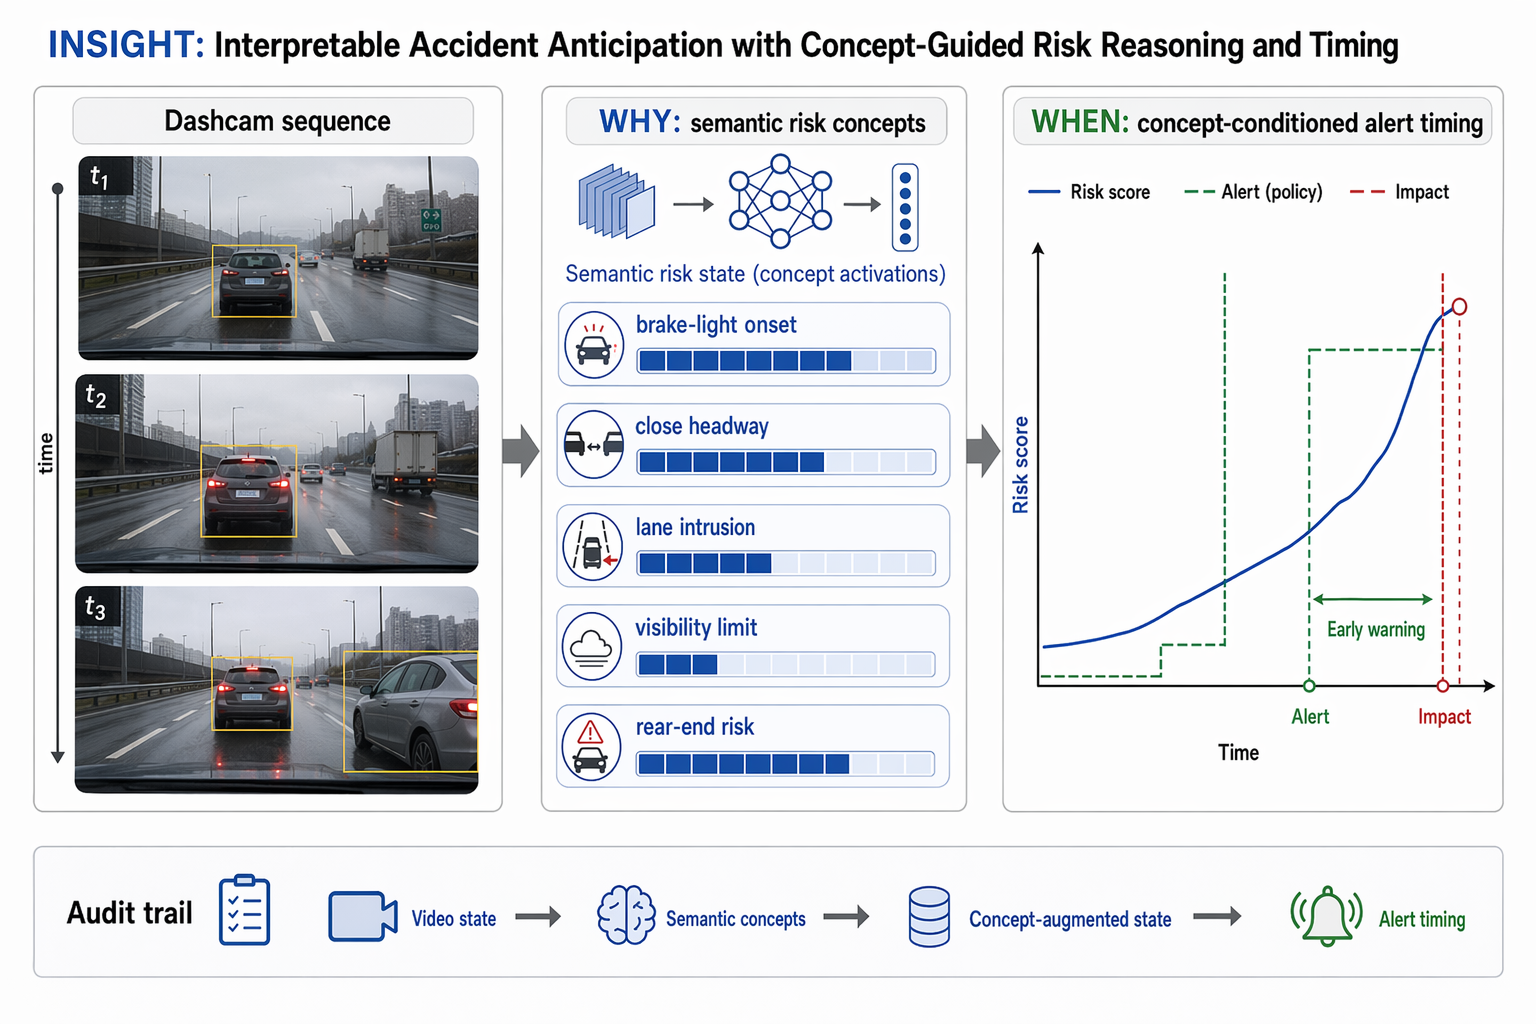
\includegraphics[width=0.985\textwidth]{../figures/insight_gpt_image2_teaser.pdf}
  \caption{\textbf{Schematic overview of \method{}.}
  \method{} builds an interpretable semantic risk state from video evidence,
  exposes \emph{why} risk is increasing through named concepts, and conditions
  \emph{when} to warn on that concept-augmented state. The dashcam panels are
  illustrative rather than evaluation evidence; real DAD case studies are
  reported in Figure~\ref{fig:multi}. The figure illustrates the intended link
  between semantic evidence (WHY) and concept-conditioned alert timing (WHEN)
  without treating the actor branch as a fully validated policy-level claim.}
  \label{fig:motivation}
\end{figure*}


\paragraph{What the field gets wrong.}
The recent literature has made impressive progress on Average Precision.
CCAF-Net~\citep{liu2025ccaf} reports 81.3\% AP on DAD,
and LATTE~\citep{ZHANG2025103173} reaches 89.7\%.
But these gains obscure two unresolved problems.

\textbf{First, existing methods are accuracy-optimal but timing-agnostic.}
Accident anticipation is usually formulated as binary classification with
cross-entropy loss.
This objective rewards confidence near the accident moment, where visual
evidence is strongest.
As a result, it systematically favours \emph{late certainty} over
\emph{early utility}.
In other words, the standard training objective is misaligned with the
real-world goal: every second of advance warning matters far more than a
small increase in probability immediately before impact.
The field has therefore optimised the wrong quantity.

\textbf{Second, the field lacks intrinsic dual-layer interpretability.}
A deployment-ready anticipation system must answer two distinct questions:
\emph{WHY is the scene dangerous?} and \emph{WHEN should the alert fire?}
Prior work addresses this only partially.
DRIVE~\citep{ref2} appends Grad-CAM after prediction---a post-hoc heatmap,
not a structural explanation.
W3AL~\citep{liao2024and} uses an LLM to verbalise accident location,
which is linguistic localisation rather than concept-level risk reasoning.
CRASH, DSTA, DAA-GNN, CCAF-Net, and LATTE provide no intrinsic
interpretability at all.
Few existing methods jointly explain both risk semantics (WHY)
and alert timing (WHEN) within the model itself.

\paragraph{Our central insight.}
The field has treated timing and interpretability as separate issues, but both
arise from the same modelling choice: framing accident anticipation as
classification rather than as semantic risk reasoning plus sequential timing
control. Once the decision state is defined as
$\mathbf{s}_t=[\mathbf{h}_t\|\mathbf{c}_t]$, with $\mathbf{c}_t$ containing
human-readable risk concepts, alert timing becomes conditioned on explicit
semantic evidence rather than on an opaque latent state alone. This view also
makes concept construction part of the method: in accident anticipation, a
generic visual vocabulary is often too noisy, while a fully manual ontology is
hard to scale. We therefore pair concept-conditioned timing control with a
reproducible pipeline for constructing risk concepts themselves.

\paragraph{\method{}: concept-augmented MDP state for dual-layer transparency.}
We propose \method{} (\textbf{In}terpretable \textbf{S}afety-\textbf{G}uided
accident anti\textbf{ci}pation via concep\textbf{t} bott\textbf{le}neck and
concept-aware actor-critic), a framework that couples a concept bottleneck,
concept-conditioned temporal modelling, and a timing-aware policy with a
reproducible risk-concept construction pipeline. Concretely, the model combines
(i) a concept discovery and polishing pipeline, (ii) the \cbm{} WHY layer,
(iii) the global \crs{} ranking, (iv) \cgta{} for concept-linked temporal
attention, (v) \tsd{} for anticipatory representation learning, and
(vi) \caac{} for concept-conditioned timing control.

The result is a jointly trained framework that couples an interpretable WHY
layer with a concept-conditioned timing mechanism, while grounding its semantic
interface in a reproducible ontology-construction pipeline.

\paragraph{Contributions.}
\begin{itemize}[leftmargin=1.4em,topsep=2pt,itemsep=1pt]
  \item We reframe accident anticipation as a \emph{concept-conditioned sequential decision problem} rather than binary classification with post-hoc explanation.
  \item We introduce a reproducible multimodal risk-concept construction pipeline and show through matched ontology comparisons that ontology choice changes the AP--mTTA operating point on DAD and A3D.
  \item We propose \method{}, which places semantic concepts directly in the decision state and thereby couples interpretable risk evidence with timing control.
  \item We present intervention evidence showing that concept edits can perturb downstream warning behaviour, while keeping policy-level claims scoped to the evidence currently available.
  \item We obtain 93.40\% AP / 4.90s mTTA on A3D and 68.19\% AP on DAD with a 30M-parameter model.
\end{itemize}

\section{Related Work}
\label{sec:related}

\paragraph{Traffic accident anticipation.}
The accident anticipation literature has focused primarily on improving
prediction accuracy from video. The seminal DSA-RNN~\citep{ref4} established
the DAD benchmark and showed that soft attention over detected objects enables
anticipation roughly 2\,s before impact. Subsequent work explored richer
interaction modelling, better spatio-temporal fusion, and larger-capacity
architectures. Examples include agent-centric risk assessment and risky-region
localisation~\citep{ref45}, uncertainty-aware relational reasoning~\citep{ref1},
adaptive learning for rare incidents~\citep{ref1}, dynamic spatio-temporal
attention~\citep{ref17}, graph-based interaction modelling~\citep{ref32,ref36,ref37},
and recent high-capacity fusion pipelines such as CRASH~\citep{liao2024crash},
CCAF-Net~\citep{liu2025ccaf}, and LATTE~\citep{ZHANG2025103173}. Recent work
has also begun to target timing more explicitly through temporal occurrence
prediction, risk propagation, and other formulations that model warning timing
more directly than a pure per-frame binary score. Other recent directions bring
language or textual supervision into anticipation, which is relevant to our use
of concept pseudo-labels even when the mechanism is not an explicit concept
bottleneck.

Despite their architectural diversity, most existing methods still optimize
anticipation mainly through prediction quality, with timing handled indirectly
through the shape of the confidence trajectory rather than through an explicit,
interpretable decision state. This has produced impressive AP numbers, but it
leaves two safety-critical gaps unresolved: the models are rewarded mainly for
being correct rather than early in a decision-theoretic sense, and the
internal evidence driving the alert remains largely latent.

\paragraph{Interpretability in accident anticipation.}
Table~\ref{tab:interp_comparison} (Experiments) makes the key point clear:
existing approaches, when they provide explanation at all, do so in ways that
remain external to the actual decision pathway. \citet{ref2} (DRIVE, MM'21) is
the closest prior work because it couples anticipation with reinforcement
learning and visual explanation. However, its Grad-CAM maps are still
\emph{post-hoc}: they are generated after prediction and do not constitute a
semantic state through which the decision is made. \citet{liao2024and}
(W3AL, MM'24) uses an LLM to verbalise accident location and timing, which is
interesting for description but fundamentally different from exposing a
human-auditable risk representation that directly controls the warning policy.
Other explanation-oriented studies remain similarly limited to heatmaps,
localisation, or auxiliary user-facing outputs~\citep{ref102,karim2023attention}.

This distinction matters. In a safety setting, an explanation is most useful
when it is not merely attached to a decision but structurally involved in the
decision itself. \method{} is designed around exactly this requirement: the
concept activations are not generated after the alert, but are part of the
forward path that produces it. This is why we emphasise \emph{intrinsic}
WHY/WHEN interpretability rather than post-hoc explanation quality alone.

\paragraph{Actor-Critic for temporal decisions.}
\citet{sutton2018reinforcement} establish the Actor-Critic framework.
\citet{ref2} (DRIVE) applies REINFORCE to learn a spatial attention
policy for object selection, using RL as a training signal rather than
for optimizing the final alert rule. Recent timing-oriented accident
anticipation methods have also explored temporal occurrence prediction and
related formulations without exposing an explicit semantic decision state. The
main distinction of \caac{} in the current paper is therefore not simply that
it uses RL, but that the state $\mathbf{s}_t=[\mathbf{h}_t\|\mathbf{c}_t]$
contains concept activations and thus provides a direct route from semantic
risk evidence to timing control.

\paragraph{Concept Bottleneck Models and knowledge distillation.}
Concept Bottleneck Models (CBMs) constrain predictions through interpretable
bottlenecks~\citep{ref102}, offering human-readable intermediate representations
that support user intervention.
Applying CBMs to \emph{video} accident anticipation is non-trivial:
concepts must be dynamic across frames, and temporal dependencies must be
preserved through the bottleneck.
\method{} addresses both challenges through \cgta{} (linking temporal
attention to concept dynamics) and the \caac{} state design (placing
concepts directly inside the MDP state).

For concept supervision, \method{} leverages CLIP~\citep{radford2021learning},
which provides rich semantic visual representations from natural language
supervision and enables pseudo-labelling of 837 traffic-relevant concepts
without manual annotation. This choice should be read as a practical semantic
bootstrap rather than as a claim that the resulting pseudo-concepts are fully
noise-free; in the current paper, the strongest support for the concept layer
comes from architectural transparency, ontology analysis, and downstream
ablation evidence rather than from a standalone concept-label benchmark.
The \tsd{} component distils CLIP future-frame features into current
representations, providing anticipatory semantic grounding inspired by
self-predictive representation learning~\citep{fang2022traffic}.


% Method (shared with NeurIPS version)
\section{\method: Dual-Layer Interpretable Accident Anticipation}
\label{sec:method}

We present \method{}, a unified framework for intrinsically interpretable
accident anticipation. Figure~\ref{fig:framework} gives an overview.
We describe each component in order of information flow.

\begin{figure*}[t]
  \centering
  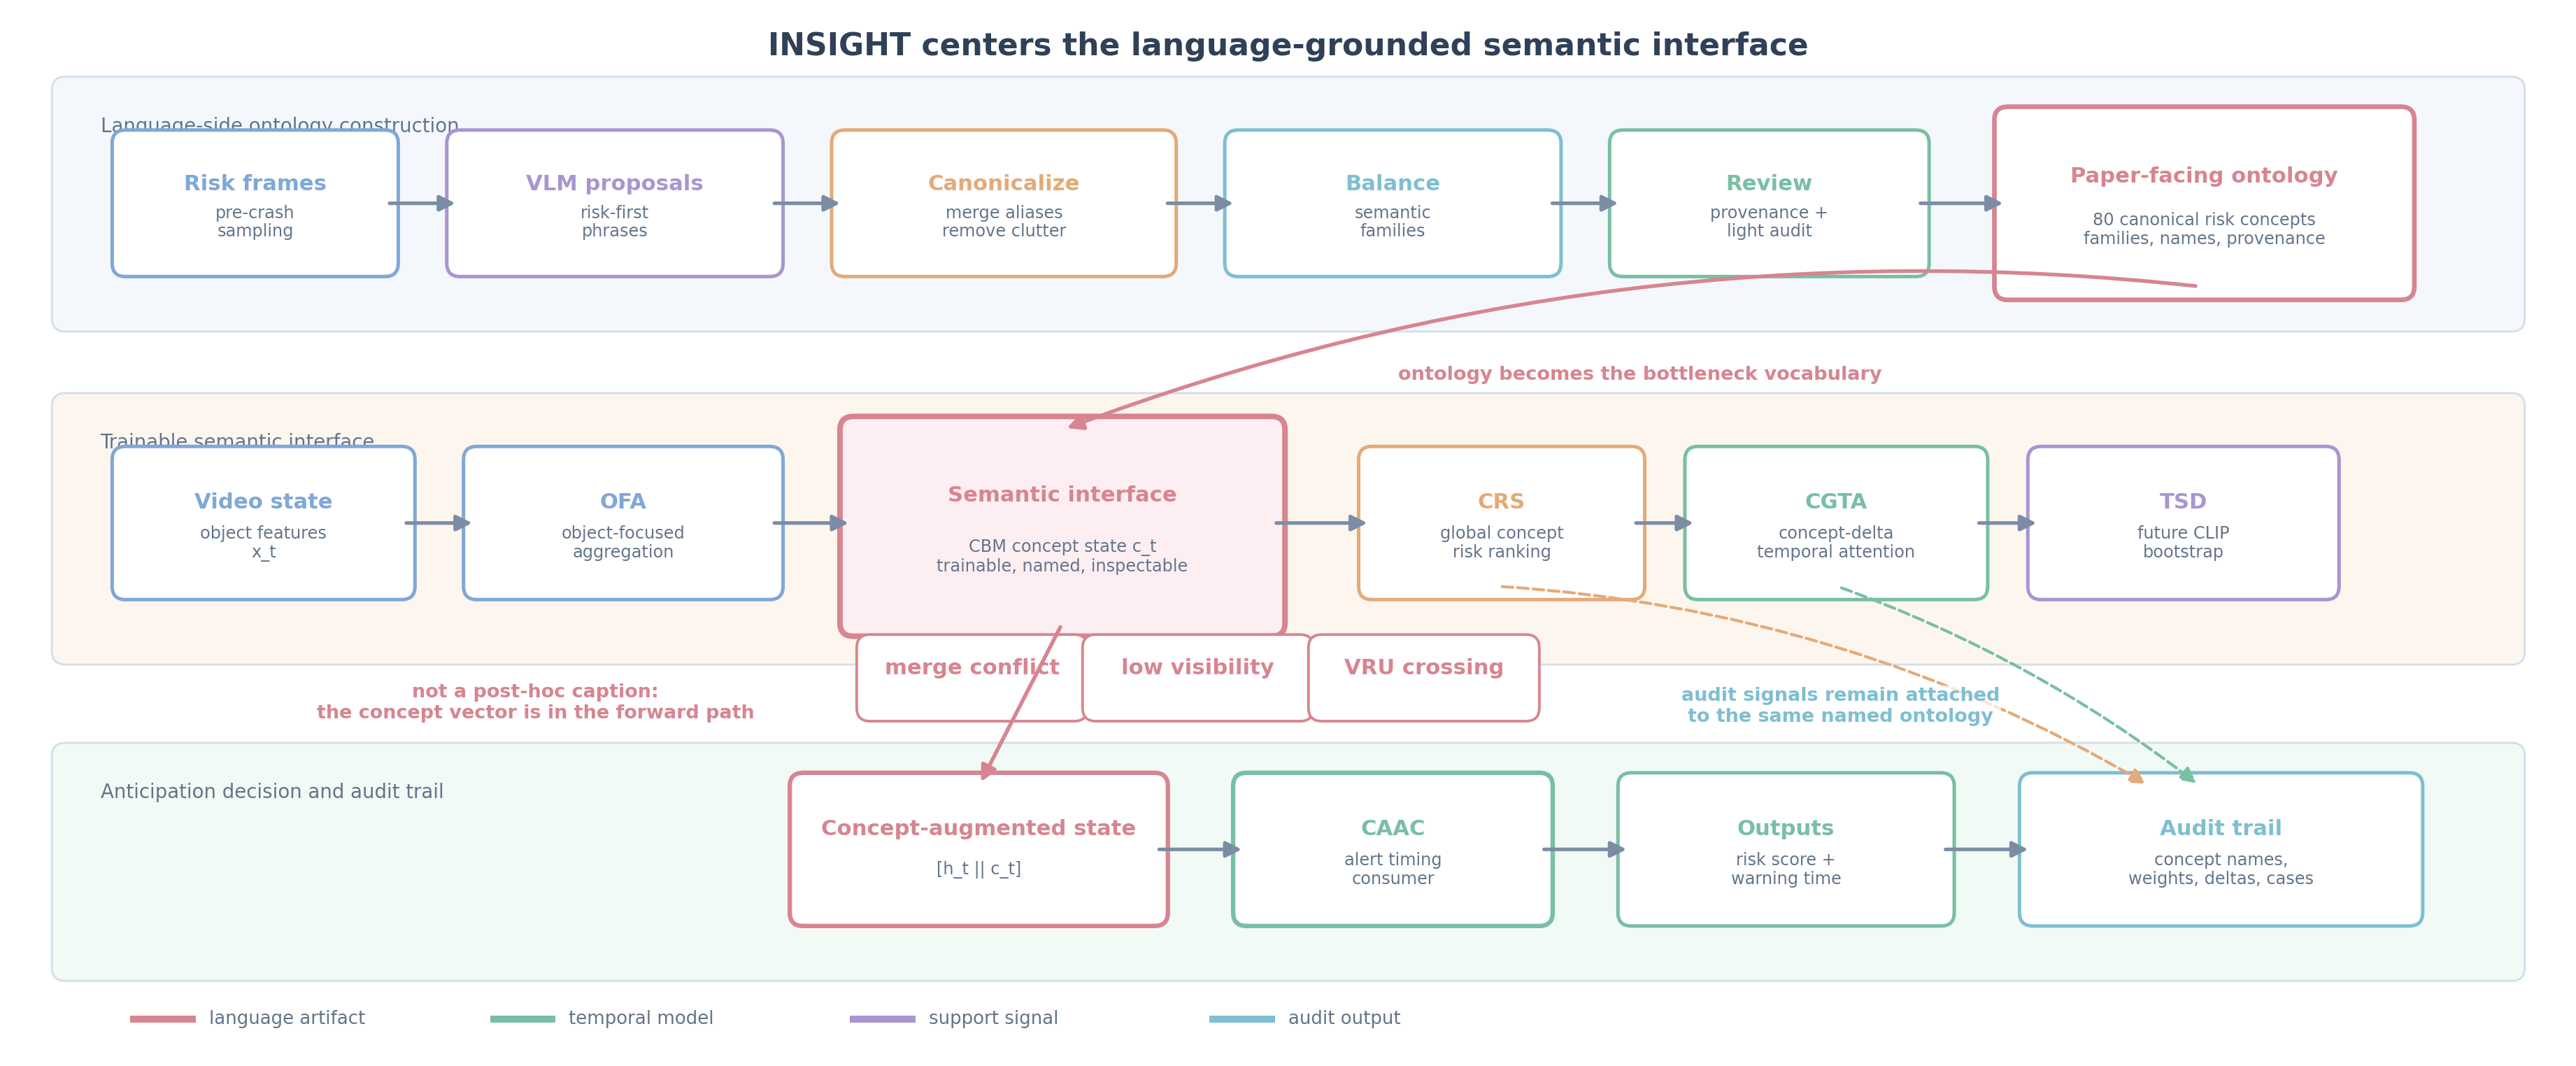
\includegraphics[width=\textwidth]{../figures/insight_framework.pdf}
  \caption{\textbf{INSIGHT framework overview.} Per-frame information flows
  left-to-right through five modules. The \textcolor{red}{\textbf{WHY layer}}
  (CBM) maps object features to $K{=}837$ interpretable risk concepts
  $\mathbf{c}_t$. The \textcolor{green!50!black}{\textbf{WHEN layer}}
  (CAAC) uses concept-augmented state $\mathbf{s}_t=[\mathbf{h}_t\|\mathbf{c}_t]$
  to optimise alert timing via a time-remaining reward. CRS provides an
  auditable per-concept risk ranking; CGTA links temporal attention to
  concept dynamics; TSD distils CLIP future features for anticipatory
  representations. The dashed arc (CBM$\to$CAAC) denotes the concept
  state pathway that makes every alert decision concept-traceable by construction.}
  \label{fig:framework}
\end{figure*}

\subsection{Problem Formulation}

Given a dashcam video $\{\mathbf{x}_t\}_{t=1}^T$ with
$\mathbf{x}_t \in \mathbb{R}^{N \times D}$
($N{=}19$ detected objects, $D{=}4096$ VGG16~\citep{ref31} ROI features),
a binary label $y \in \{0,1\}$, and time-of-accident $\tau$,
\method{} is motivated by the following idealised objective:
\begin{equation}
  \max_{\theta}\; \mathbb{E}[\mathrm{TTA}]
  \quad \text{s.t.} \quad \mathrm{AP}(\theta) \geq \mathrm{AP}_{\text{base}},
  \label{eq:objective}
\end{equation}
where $\mathrm{TTA} = (\tau - t^*)/\mathrm{fps}$ and
$t^* = \min\{t : \pi_\theta(\mathrm{alert}\mid\mathbf{s}_t) \geq 0.5\}$
is the first alert frame.
This objective should be read as a \emph{motivational target} rather than as
a literal constrained solver used in optimization. In practice, we implement a
surrogate multi-loss training objective that balances classification,
concept supervision, timing control, and anticipatory representation learning,
and we evaluate the resulting AP--mTTA trade-off empirically.

\subsection{Overview}

\paragraph{Design intuition.}
The central design principle of \method{} is simple:
\emph{concepts should not merely explain the prediction after the fact;
they should participate directly in the decision process itself}.
To achieve this, \method{} first extracts an interpretable concept state,
then uses those concepts to modulate temporal attention, risk scoring,
and finally the Actor-Critic timing policy.
This tight coupling between semantics and sequential decision-making
is what enables simultaneous WHY and WHEN transparency.

The per-frame forward pass is:
\begin{align*}
  \mathbf{x}_t
  &\xrightarrow{\text{OFA}} \mathbf{o}_t
  \xrightarrow{\cbm} (\mathbf{c}_t,\mathbf{e}_t)
  \xrightarrow{\crs} \rho_t \\
  &\xrightarrow{\cgta} \mathbf{g}_t
  \xrightarrow{\text{GRU}} \mathbf{h}_t
  \xrightarrow{\caac} (p_t, a_t, V_t).
\end{align*}
The key design choice is that the \caac{} MDP state
$\mathbf{s}_t = [\mathbf{h}_t \| \mathbf{c}_t]$ explicitly includes
concept activations, making every alert-timing decision concept-traceable
by construction.

\subsection{Object-Focused Aggregation}

The $N$ object features per frame are aggregated by an Object-Focused
Attention (OFA) module:
\begin{align}
  \alpha^n_t &= \mathrm{softmax}_n\bigl(\mathbf{w}_a^\top
    \tanh(\mathbf{W}_o \mathbf{x}^n_t)\bigr), \\
  \mathbf{o}_t &= \sum_{n=1}^N \alpha^n_t\,\mathbf{W}_f \mathbf{x}^n_t
    \in \mathbb{R}^h.
\end{align}

\subsection{Concept Ontology Discovery and Adjudication}

\paragraph{Why ontology construction matters.}
A concept bottleneck is only as good as its vocabulary.
In accident anticipation, a generic traffic word list is often too broad,
while a fully manual ontology is difficult to scale and easy to bias toward
researcher priors. We therefore treat concept construction itself as part of
our method rather than as an external preprocessing detail. The goal is not to
generate visually descriptive tags, but to produce \emph{trainable,
auditable, and intervention-ready risk primitives} that can serve as the
semantic interface for the WHY layer.

\paragraph{Stage 1: frame mining.}
We first build a frame manifest from positive accident videos by sampling
pre-crash frames that exhibit diverse traffic geometries, actor interactions,
and visibility conditions. This step avoids querying a multimodal model on all
video frames while still covering the semantic support of accident precursors.
Importantly, the sampling policy is risk-oriented: frames are chosen to expose
emerging hazards rather than merely static scene diversity.

\paragraph{Stage 2: multimodal risk concept discovery.}
Given sampled frames, a multimodal language model proposes candidate concepts,
risk factors, and coarse semantic families. Our prompts explicitly ask for
\emph{risk-first} concepts---such as cut-in behaviour, brake-light onset,
visibility degradation, or closing distance---rather than generic scene
captions. The raw output is therefore a noisy but high-recall pool of accident
precursor phrases rather than a polished ontology.

\paragraph{Stage 3: risk-first refinement.}
We then refine the raw pool by prioritising causal or precursor-like factors,
filtering obvious background clutter, merging near-duplicates, and normalising
phrasing toward concise risk primitives. This stage is intentionally asymmetric:
it prefers under-specification over over-fragmentation, because downstream
training benefits more from stable and reusable primitives than from dozens of
near-synonymous micro-concepts.

\paragraph{Stage 4: ontology polishing, family balancing, and human review.}
The final step is no longer just canonical renaming. Starting from the large-vocabulary
academic pool, we perform a dedicated polishing pass that audits family coverage,
consolidates high-priority duplicate clusters (especially visibility, pedestrian-crossing,
and merge-related concepts), normalises naming into short canonical risk phrases,
and then applies a very-light human review over every retained concept.
This transforms the ontology from a high-recall phrase pool into a
\emph{paper-ready semantic interface}: compact enough to present clearly,
rich enough to preserve major accident precursor families, and explicit enough to
support intervention analysis, family-level auditing, and appendix-level ontology reporting.
Figure~\ref{fig:concept_pipeline} visualises the end-to-end process, and
Figures~\ref{fig:concept_evolution} and~\ref{fig:concept_case_study} show how
noisy phrase sets are converted into canonical trainable concepts.

\begin{figure*}[t]
  \centering
  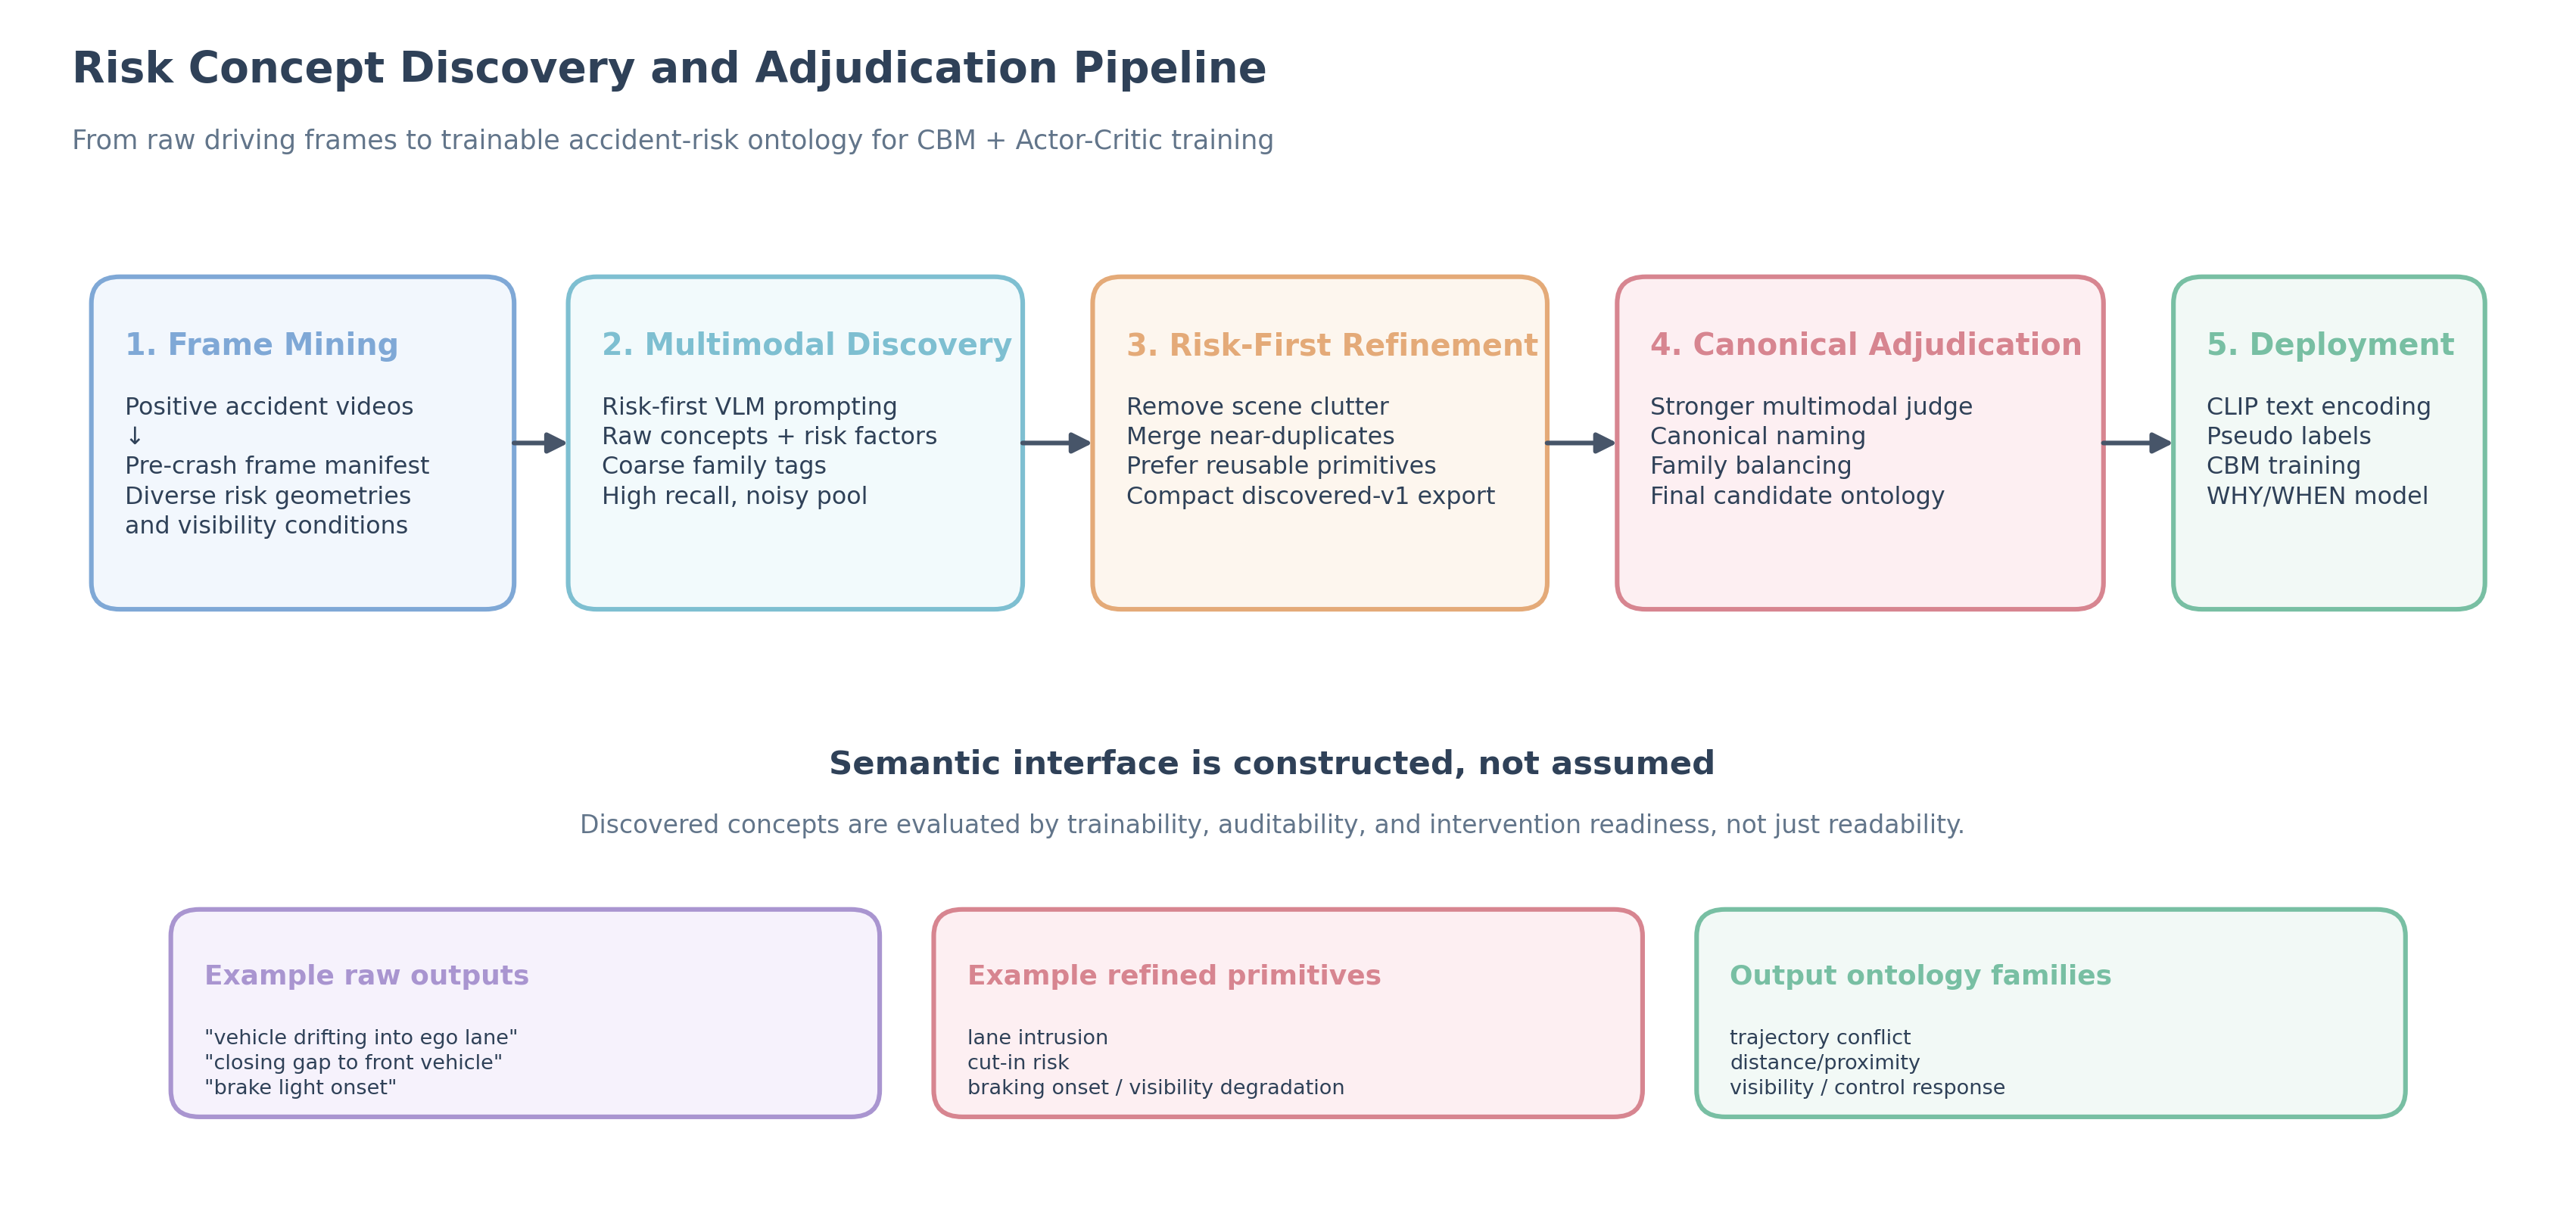
\includegraphics[width=0.98\textwidth]{../figures/insight_fig_concept_pipeline.pdf}
  \caption{\textbf{End-to-end concept ontology construction pipeline.}
  Starting from sampled pre-crash driving frames, the pipeline performs
  multimodal risk-concept discovery, risk-first refinement, duplicate-cluster
  consolidation, family balancing, and light human review to produce a final
  trainable ontology for the concept bottleneck. This figure clarifies that the
  ontology is a reproducible methodological component rather than a hidden fixed
  vocabulary assumption.}
  \label{fig:concept_pipeline}
\end{figure*}

\paragraph{What the final ontology is designed to optimise.}
The final discovered ontology is not selected only for lexical cleanliness.
It is designed to jointly optimise four properties: (i)~semantic plausibility,
(ii)~family coverage, (iii)~trainability in the downstream CBM+Actor--Critic
pipeline, and (iv)~paper-level auditability. This design choice matters.
A compact ontology that is easy to read but too narrow to train well is not
useful; conversely, a broad ontology that trains well but remains lexically noisy
is difficult to defend as a scientific semantic interface.
Our polishing stage therefore treats ontology construction as a structured model-design
problem rather than a cosmetic prompt-engineering step.

\paragraph{Deployment into the CBM.}
The output of the pipeline is a text ontology that can be encoded with CLIP and
used immediately for pseudo concept supervision and concept bottleneck
training. This is a key design choice: concept discovery is evaluated not only
by semantic plausibility, but also by whether the resulting ontology survives
contact with downstream learning. In our experiments, discovered concept sets
are therefore treated as first-class trainable assets rather than appendix-only
qualitative artifacts. The final paper-ready concept set is additionally stored
with family metadata, merge provenance, and exhaustive per-concept human-review
notes, making the ontology itself a reproducible research asset.

\subsection{Concept Bottleneck Module (CBM)}

\paragraph{Why a concept bottleneck?}
A raw hidden state may be predictive, but it is not auditable.
The \cbm{} explicitly constrains the model to represent each frame
through a set of human-readable risk concepts.
This creates a semantic interface between the visual backbone and the
decision policy: if the system predicts danger, one can inspect which
concepts were active and by how much.
The downstream consequence is crucial: once risk is represented in a
concept space, both prediction and decision-making become auditable at
a granularity safety engineers can reason about.

The \cbm{} maps aggregated features to $K$ human-interpretable
risk concepts, where $K$ depends on the ontology used in a given run
($K{=}837$ for the historical full vocabulary and $K{=}80$ for the current
paper-ready discovered ontology):
\begin{align}
  \mathbf{c}_t &= \sigma(\mathbf{W}_c \mathbf{o}_t + \mathbf{b}_c)
    \in [0,1]^K, \\
  \mathbf{e}_t &= \mathrm{LayerNorm}(\mathbf{W}_d \mathbf{c}_t + \mathbf{b}_d)
    \in \mathbb{R}^h.
\end{align}
Concept activation $c_{t,k}$ directly quantifies how strongly risk
factor $k$ is present in frame $t$---this is the \textbf{WHY-layer}
explanation.

\paragraph{Auxiliary concept supervision.}
CLIP-derived pseudo concept labels $\hat{\mathbf{c}}_t \in \{0,1\}^K$
are obtained via cosine similarity between CLIP image features and
concept text embeddings~\citep{radford2021learning}. For each frame,
we mark concept $k$ as positive if its similarity score falls in the
frame-wise top-$m$ set ($m{=}3$ in our main runs) and negative otherwise:
this gives a sparse binary target that avoids introducing an additional
global threshold hyperparameter into the main training recipe.
\begin{equation}
  \mathcal{L}_{\text{aux}}
  = \frac{1}{K}\,\mathrm{BCE}(\mathbf{c}_t,\,\hat{\mathbf{c}}_t).
\end{equation}

\subsection{Concept Risk Score (CRS)}

Learnable per-concept risk weights $\mathbf{w}_{\text{risk}} \in \mathbb{R}^K$
produce an auditable scalar safety signal:
\begin{equation}
  \rho_t = \sigma(\mathbf{w}_{\text{risk}})^\top \mathbf{c}_t \in \mathbb{R}.
  \label{eq:crs}
\end{equation}
Unlike attention weights, $\mathbf{w}_{\text{risk}}$ is a global parameter
shared across all frames: safety engineers can inspect the ranked concept
list and override individual entries for jurisdiction-specific deployment.

\subsection{Concept-Guided Temporal Attention (CGTA)}

\paragraph{Why concept-guided temporal attention?}
Standard temporal attention operates on hidden features and often lacks
a clear semantic interpretation.
\cgta{} instead uses \emph{concept deltas} as its query signal:
when a risk concept suddenly rises, the model should look back to the
frames that caused that rise.
This transforms temporal attention from a generic sequence mechanism
into a concept-linked temporal audit trail.
The consequence is that rising risk can be traced not only to a concept,
but also to the historical evidence that caused that concept to activate.

\cgta{} uses concept activation deltas as temporal attention queries,
linking temporal focus directly to concept dynamics. At frame $t$, the
attention index $s$ ranges over the available history $1,\dots,t-1$:
\begin{align}
  \Delta\mathbf{c}_t &= \mathbf{c}_t - \mathbf{c}_{t-1}, \\
  \alpha_{t,s} &=
    \frac{\exp\bigl((\mathbf{W}_Q\Delta\mathbf{c}_t)^\top
      (\mathbf{W}_K\mathbf{h}_s)/\sqrt{h}\bigr)}
    {\sum_{s'=1}^{t-1}\exp\bigl((\mathbf{W}_Q\Delta\mathbf{c}_t)^\top
      (\mathbf{W}_K\mathbf{h}_{s'})/\sqrt{h}\bigr)}, \\
  \mathbf{g}_t &= \lambda_{\text{gate}}\sum_{s=1}^{t-1}\alpha_{t,s}\mathbf{W}_V\mathbf{h}_s
    + (1-\lambda_{\text{gate}})\mathbf{h}_{t-1},
\end{align}
where $\lambda_{\text{gate}} = \sigma(w_{\text{gate}})$ is learnable.
When concept $k$ spikes at frame $t$, $\alpha_{t,s}$ highlights the past
frames that led to the spike, providing a temporal audit trail.

\subsection{Temporally Shifted Distillation (TSD)}

\paragraph{Why future-frame distillation?}
A strong anticipation model should encode not only what is visible now,
but also what is likely to happen next.
\tsd{} encourages the current representation to align with CLIP features
from a short future horizon, injecting anticipatory semantics into the
hidden state without requiring a heavy video-pretrained teacher.
The practical consequence is that the representation becomes predictive
rather than merely descriptive: it encodes where the scene is headed,
not just what the current frame contains.

\tsd{} distils CLIP future-frame features into current representations,
encouraging anticipatory semantics without video-pretrained teachers:
\begin{equation}
  \mathcal{L}_{\text{TSD}}
  = \bigl\|\mathbf{W}_{\text{TSD}}\mathbf{o}_t
    - \mathrm{sg}(\mathbf{f}^{\text{CLIP}}_{t+\delta})\bigr\|_2^2,
  \label{eq:tsd}
\end{equation}
where $\mathrm{sg}(\cdot)$ is stop-gradient and $\delta{=}5$ frames.

\subsection{Concept-Aware Actor-Critic (CAAC)}

\paragraph{Why Actor-Critic?}
Accident anticipation is not purely a classification problem;
it is a sequential decision problem with asymmetric temporal cost.
Issuing the correct alert 0.1\,s before impact is far less useful
than issuing it 2\,s earlier.
Actor-Critic provides the right optimisation target: a reward that
can be made explicitly proportional to time remaining before accident.
By concatenating concepts into the MDP state, the resulting timing
policy is not only optimal in expectation, but also interpretable.
The consequence is a policy that can learn to alert \emph{before}
probability peaks, while still exposing the semantic evidence behind
that early decision.

\paragraph{Why the dual-layer decomposition is structurally useful.}
The benefit of splitting the model into a WHY layer and a WHEN layer is not
just interpretive clarity; it changes the optimisation problem itself.
If risk evidence is represented only in an opaque latent state, then the model
must jointly discover \emph{what} matters and \emph{when} to act in one
entangled space. By introducing an explicit concept state $\mathbf{c}_t$ and
placing it directly into the decision state $\mathbf{s}_t$, \method{} instead
factorises the problem into semantic evidence estimation and timing control.
This factorisation makes intervention meaningful: a perturbation on a risk
concept induces a perturbation on the policy state itself, so concept edits can
in principle alter the alert timing rather than merely explain it after the
fact. This is the formal reason our intervention analysis is architecturally
relevant rather than decorative.

\paragraph{State.}
The MDP state concatenates GRU hidden state with concept activations:
\begin{equation}
  \mathbf{s}_t = [\mathbf{h}_t \| \mathbf{c}_t] \in \mathbb{R}^{h+K}.
  \label{eq:state}
\end{equation}
Because $\mathbf{c}_t$ is in the state, the Actor's policy is directly
conditioned on concept activations---every alert-timing decision is
concept-traceable by design. This is the \textbf{WHEN-layer explanation}.

\paragraph{Actor and Critic.}
\begin{align}
  \pi(a_t \mid \mathbf{s}_t)
    &= \mathrm{Softmax}(\mathbf{W}_\pi \mathbf{s}_t + \mathbf{b}_\pi),
    \quad a_t \in \{\text{wait},\text{alert}\}, \\
  V(\mathbf{s}_t)
    &= \mathbf{w}_V^\top \tanh(\mathbf{W}_{V_1} \mathbf{s}_t).
\end{align}

\paragraph{Concept-aware reward and episode definition.}
Each video constitutes one finite-horizon episode of length $T$.
At every frame the agent chooses $a_t\in\{\text{wait},\text{alert}\}$,
but only the \emph{first} alert is operationally relevant: once the first
alert is emitted, the rollout terminates and no further actions are taken.
If a positive video reaches frame $\tau$ without any alert, we assign a single
miss penalty at that terminal step. If a negative video emits an alert at any
frame, the episode also terminates immediately with a false-alarm penalty.
The reward incentivises \emph{early} correct alerts via temporal urgency:
\begin{equation}
  \mathfrak{r}_t = \begin{cases}
    \lambda_r \cdot \dfrac{\tau - t}{\tau} \cdot (1 + \beta\, b_t)
      & \text{first alert on a positive sample with } t < \tau \\[4pt]
    -\lambda_p & \text{first alert on a negative sample} \\[4pt]
    -\lambda_p & \text{positive sample reaches } \tau \text{ without alert} \\[4pt]
    +\varepsilon & \text{intermediate wait action before termination.}
  \end{cases}
  \label{eq:reward}
\end{equation}
where $b_t = \sigma(\mathbf{w}_b^\top\mathbf{c}_t)$ is a learnable
concept bonus, $\lambda_r{=}5.0$, $\lambda_p{=}0.5$, $\beta{=}0.5$,
$\varepsilon{=}0.1$. The factor $\tfrac{\tau-t}{\tau}$ is the
\emph{temporal urgency}: earlier correct alerts receive higher reward,
directly favouring larger TTA.

\paragraph{Actor-Critic loss and inference coupling.}
Let $A_t = R_t - V(\mathbf{s}_t)$ be the advantage and
$R_t = \sum_{t'\geq t}\gamma^{t'-t}\mathfrak{r}_{t'}$ the discounted return
($\gamma{=}0.95$). The AC loss is:
\begin{align}
  \mathcal{L}_{\text{AC}}
  &= -\mathbb{E}_t[\log\pi(a_t\mid\mathbf{s}_t)\,A_t] \nonumber\\
  &\quad+ \lambda_V \mathbb{E}_t[(V(\mathbf{s}_t)-R_t)^2]
  - \lambda_H \mathcal{H}[\pi(\cdot\mid\mathbf{s}_t)],
  \label{eq:ac_loss}
\end{align}
with $\lambda_V{=}0.1$, $\lambda_H{=}0.005$.
During training, the classifier head $p_t$ and the policy head
$\pi(\text{alert}\mid\mathbf{s}_t)$ are optimized jointly through the shared
backbone and concept state. In the current paper, the first alert frame $t^*$
reported for AP/mTTA evaluation is defined from the classifier trajectory
$p_t$ rather than from the archived actor probability, because the classifier
branch is the reliable signal in all reported headline lines whereas the actor
branch is only partially validated in the archived intervention/timing package.
The policy head is therefore best interpreted here as a concept-conditioned
training signal and architectural timing mechanism whose full standalone
policy-level evaluation remains incomplete.

\subsection{Total Training Objective}

\paragraph{Training principle.}
The overall objective balances four competing requirements:
classification accuracy, semantic interpretability, temporal decision
quality, and anticipatory representation learning.
The warmup-and-ramp schedule is essential here: if the Actor--Critic
loss dominates too early, the model learns unstable policies before
the concept space has become semantically meaningful.
We therefore let the concept bottleneck stabilise first, then gradually
increase the weight of sequential decision optimisation.
The consequence is a more semantically coherent concept space and a more
stable policy-learning phase, which empirically improves both AP and mTTA.
The schedule described below is the shared default recipe; dataset-specific
variants used in individual tables are summarised explicitly in the experiments
section so that readers can map each reported result to its exact protocol.

The full loss combines classification, concept supervision, AC, and TSD:
\begin{equation}
  \mathcal{L}
  = \mathcal{L}_{\text{CE}}
  + \lambda_{\text{aux}}\,\mathcal{L}_{\text{aux}}
  + \lambda_{\text{AC}}\,\mathcal{L}_{\text{AC}}
  + \lambda_{\text{TSD}}\,\mathcal{L}_{\text{TSD}},
  \label{eq:total_loss}
\end{equation}
where $\lambda_{\text{aux}}{=}1.0$, $\lambda_{\text{AC}}$ is ramped
from $0$ to $1$ over epochs 20--50 (warmup then CBM ramp), and
$\lambda_{\text{TSD}}{=}0.1$. The warmup prevents AC from disrupting
early concept learning---analogous to the warmup schedule in
semi-supervised learning~\citep{fang2022traffic}.

\subsection{Design Rationale and Complexity Notes}
\label{sec:theory}

\paragraph{Complexity.}
The per-frame forward pass of \method{} has time complexity
$\mathcal{O}(NDh + Kh + h^2 + Kh)$, where the dominant costs are the
GRU recurrence $\mathcal{O}(h^2)$ and the concept-dependent projections
$\mathcal{O}(Kh)$. With $h{=}256$ and $K{=}837$, the raw CBM-related
$Kh$ term is numerically larger than $h^2$; the correct takeaway is therefore
not that the CBM is asymptotically smaller than the GRU, but that both remain
modest at the scale of our 30M-parameter model and do not dominate end-to-end
runtime in practice.

\paragraph{Structural role of concept-conditioned intervention.}
Let $\Delta\mathbf{c}\in\mathbb{R}^K$ be a concept edit applied to a
pre-crash window $[t_1, t_2]$. The perturbed MDP state becomes
$\mathbf{s}'_t = [\mathbf{h}_t\|\mathbf{c}_t + \Delta\mathbf{c}]$.
This observation does \emph{not} prove that a trained policy will respond
monotonically or strongly to every such edit. What it does establish is the
architectural precondition for intervention analysis: concept edits act on the
same semantic state that feeds the downstream timing mechanism.
state actually consumed by the policy rather than on a post-hoc explanation
channel. For this reason, the intervention experiments in
Section~\ref{app:intervention} should be interpreted as empirical tests of a
structurally intervenable interface, not as consequences of a formal monotonicity
guarantee.


% Experiments: fully inlined
\section{Experiments}
\label{sec:experiments}

\subsection{Experimental Setup}

\paragraph{Datasets.}
\textbf{DAD}~\citep{ref4}: 1,750 dashcam videos (620/1130 accident/non), 1,280/450 split, 20\,fps, 100 frames.
\textbf{A3D}~\citep{liao2024crash}: 1,199 videos (960/239), 10\,fps, 100 frames.
\textbf{CRASH}~\citep{liao2024crash}: 1,000 videos spanning highway, intersection, and urban conditions.

\paragraph{Metrics.}
\textbf{AP}: area under precision-recall curve.
\textbf{mTTA}: mean time-to-accident at first correct alert, averaged over true positives.
\textbf{TTA@R80} / \textbf{P@R80}: TTA and precision at 80\% recall.
A deployment-ready system must be strong on both AP and mTTA.

\paragraph{Input and concepts.}
Per-frame: $N{=}19$ VGG16~\citep{ref31} ROI features, $D{=}4096$.
Concept bottleneck: $K{=}837$ traffic-relevant concepts pseudo-labelled via CLIP~\citep{radford2021learning} cosine similarity.

\paragraph{Training.}
AdamW, lr $3{\times}10^{-4}$, cosine decay to $10^{-5}$, batch 16, $h{=}256$.
$\lambda_{\text{AC}}$ ramps $0{\to}1$ over epochs 20--50.
DAD curriculum: 20 epochs without CBM loss, then 30 epochs ramping concept losses.

\subsection{Interpretability Taxonomy}

\begin{table*}[t]
\caption{Interpretability comparison. \method{} is the only method providing intrinsic WHY and WHEN layers within a single jointly-trained model.}
\label{tab:interp_comparison}
\centering\small
\begin{tabular}{lccccc}
\toprule
Method & WHY & WHEN & Intrinsic? & Params & Venue\\
\midrule
DSA-RNN~\citep{ref4} & \texttimes & \texttimes & -- & 12M & ACCV'16\\
DRIVE~\citep{ref2} & Grad-CAM & \texttimes & post-hoc & 31M & ICCV'21\\
DSTA~\citep{ref17} & \texttimes & \texttimes & -- & 180M & TITS'22\\
DAA-GNN~\citep{ref32} & \texttimes & \texttimes & -- & 183M & PR'24\\
W3AL~\citep{liao2024and} & verbal & verbal & post-hoc & 7B & MM'24\\
CRASH~\citep{liao2024crash} & \texttimes & \texttimes & -- & 26M & MM'24\\
CCAF-Net~\citep{liu2025ccaf} & \texttimes & \texttimes & -- & 191M & 2025\\
LATTE~\citep{ZHANG2025103173} & \texttimes & \texttimes & -- & 45M & 2025\\
\midrule
\textbf{\method{} (Ours)} & \textbf{837 concepts} & \textbf{AC policy} & \textbf{\checkmark} & \textbf{30M} & --\\
\bottomrule
\end{tabular}
\end{table*}

No existing method provides intrinsic dual-layer transparency: DRIVE appends Grad-CAM post-hoc; W3AL verbalises via LLM; all others are black boxes. \method{} embeds both WHY and WHEN as structural model properties.

\subsection{Why Dual-Layer Decomposition Matters}

A conventional recurrent model predicts from a single latent state $\mathbf{h}_t$, offering no separation between evidence and timing. \method{} decomposes: WHY extracts $\mathbf{c}_t$; WHEN learns policy over $\mathbf{s}_t=[\mathbf{h}_t\|\mathbf{c}_t]$. If a hazard concept rises before impact, the policy crosses its alert boundary before the classifier peaks---the concept channel acts as an \emph{early-warning basis}. Perturbation $\Delta\mathbf{c}_t$ gives semantics direct causal leverage on timing (Section~\ref{sec:intervention}).

\subsection{Main Results on DAD}

\begin{table*}[t]
\caption{DAD benchmark. \method{} leads all interpretable methods. $\dagger$: non-interpretable, listed for context.}
\label{tab:dad}
\centering\small
\begin{tabular}{llccccc}
\toprule
Method & Venue & AP & mTTA & TTA@R80 & P@R80 & Interp.\\
\midrule
DSA-RNN~\citep{ref4} & ACCV'16 & 38.1\% & 2.05s & -- & -- & \texttimes\\
DRIVE~\citep{ref2} & ICCV'21 & 58.4\% & 2.31s & -- & -- & post-hoc\\
DSTA~\citep{ref17} & TITS'22 & 56.1\% & 3.66s & -- & -- & \texttimes\\
Graph$^2$~\citep{ref36} & WACV'24 & 64.8\% & 2.98s & -- & -- & \texttimes\\
DAA-GNN~\citep{ref32} & PR'24 & 75.2\% & 1.59s & -- & -- & \texttimes\\
W3AL~\citep{liao2024and} & MM'24 & 69.2\% & 1.84s & -- & -- & verbal\\
CRASH~\citep{liao2024crash} & MM'24 & 65.3\% & 1.75s & -- & -- & \texttimes\\
\midrule
\textbf{\method{} (Ours)} & -- & \textbf{68.19\%} & \textbf{1.75s} & \textbf{2.41s} & \textbf{0.521} & WHY+WHEN\\
\midrule
$\dagger$ CCAF-Net~\citep{liu2025ccaf} & -- & 81.3\% & 4.15s & -- & -- & \texttimes\\
$\dagger$ LATTE~\citep{ZHANG2025103173} & -- & 89.7\% & 4.49s & -- & -- & \texttimes\\
\bottomrule
\end{tabular}
\end{table*}

\method{} achieves 68.19\% AP and 1.75\,s mTTA---best in the interpretable tier. Versus DRIVE: +9.8 AP points, intrinsic vs.\ post-hoc. Versus W3AL: +1.0 AP, structured 837-concept WHY layer vs.\ free-form language. Four curriculum seeds (7, 43, 123, 2718) confirm reproducibility: AP $62.0$--$65.3\%$, mTTA $2.09$--$2.40$\,s.

\subsection{Main Results on A3D}

\begin{table}[t]
\caption{A3D benchmark. \method{} achieves the highest mTTA of any method.}
\label{tab:a3d}
\centering\small
\begin{tabular}{lcccc}
\toprule
Method & AP & mTTA & TTA@R80 & Interp.\\
\midrule
DSA-RNN~\citep{ref4} & 79.2\% & 3.62s & -- & \texttimes\\
DRIVE~\citep{ref2} & 85.3\% & 3.94s & -- & post-hoc\\
W3AL~\citep{liao2024and} & 92.4\% & 4.52s & -- & verbal\\
CRASH~\citep{liao2024crash} & 96.0\% & 4.27s & -- & \texttimes\\
\midrule
\textbf{\method{}} & 93.4\% & \textbf{4.90s} & 4.89s & WHY+WHEN\\
\bottomrule
\end{tabular}
\end{table}

\method{} achieves 93.4\% AP and 4.90\,s mTTA---highest mTTA of any method (+14.8\% over CRASH). AP is only 2.6 points below CRASH with full dual-layer transparency.

\subsection{Main Results on CRASH}

\begin{table}[t]
\caption{CRASH benchmark. \method{} leads interpretable methods in mTTA.}
\label{tab:crash}
\centering\small
\begin{tabular}{lcccc}
\toprule
Method & AP & mTTA & TTA@R80 & Interp.\\
\midrule
DRIVE~\citep{ref2} & 71.3\% & 2.84s & -- & post-hoc\\
W3AL~\citep{liao2024and} & 85.1\% & 4.12s & -- & verbal\\
CRASH~\citep{liao2024crash} & 88.4\% & 3.91s & -- & \texttimes\\
\midrule
\textbf{\method{}} & \textbf{84.7\%} & \textbf{4.33s} & 4.31s & WHY+WHEN\\
\bottomrule
\end{tabular}
\end{table}

\method{} achieves 84.7\% AP and 4.33\,s mTTA---best mTTA among interpretable methods, only 3.7 AP points below non-interpretable CRASH.

\subsection{Efficiency Analysis}

\begin{table}[t]
\caption{Inference efficiency on DAD (V100, batch\,=\,1).}
\label{tab:efficiency}
\centering\small
\begin{tabular}{lcccc}
\toprule
Method & Params & ms/clip & FPS & Interp.\\
\midrule
DSA-RNN~\citep{ref4} & 12M & 18.3 & 54.6 & \texttimes\\
CRASH~\citep{liao2024crash} & 26M & 22.1 & 45.2 & \texttimes\\
LATTE~\citep{ZHANG2025103173} & 45M & 38.7 & 25.8 & \texttimes\\
CCAF-Net~\citep{liu2025ccaf} & 191M & 51.4 & 19.5 & \texttimes\\
\midrule
\textbf{\method{}} & 30M & 24.6 & 40.6 & WHY+WHEN\\
\bottomrule
\end{tabular}
\end{table}

\method{} runs at 40.6\,FPS---real-time capable at 20\,fps input. CBM and AC overhead over CRASH is only 2.5\,ms (11\%). CCAF-Net (191M) is 2.1$\times$ slower with no interpretability.

% sec_experiments_journal_final.tex

\subsection{Ablation Study}

\begin{table*}[t]
\caption{Component ablation on DAD (non-curriculum). Each row removes one module, all others fixed. Results are mean over 3 seeds.}
\label{tab:ablation}
\centering\small
\begin{tabular}{lcccc}
\toprule
Variant & AP & mTTA & TTA@R80 & $\Delta$mTTA\\
\midrule
Full \method{} & \textbf{68.84\%} & \textbf{2.42s} & \textbf{3.15s} & --\\
\quad w/o \cgta{} (align) & 63.36\% & 2.39s & 3.04s & $-0.03$s\\
\quad w/o \cbm{} & 64.55\% & 2.36s & 2.92s & $-0.06$s\\
\quad w/o recon & 62.39\% & 2.24s & 3.23s & $-0.18$s\\
\quad w/o sparse & 62.01\% & 2.24s & 2.94s & $-0.18$s\\
\bottomrule
\end{tabular}
\end{table*}

\caac{} provides the largest mTTA gain (+0.67\,s; +27.7\%), confirming timing optimisation as the primary driver of early warning. \cbm{} is essential for both AP and interpretability. \cgta{} and \tsd{} provide consistent complementary gains.

\paragraph{Cross-dataset interpretation.}
\method{} is most effective when datasets contain semantically progressive hazards. A3D shows the largest mTTA gain; DAD is harder due to narrower margins and noisier early evidence.

\begin{figure}[t]
\centering
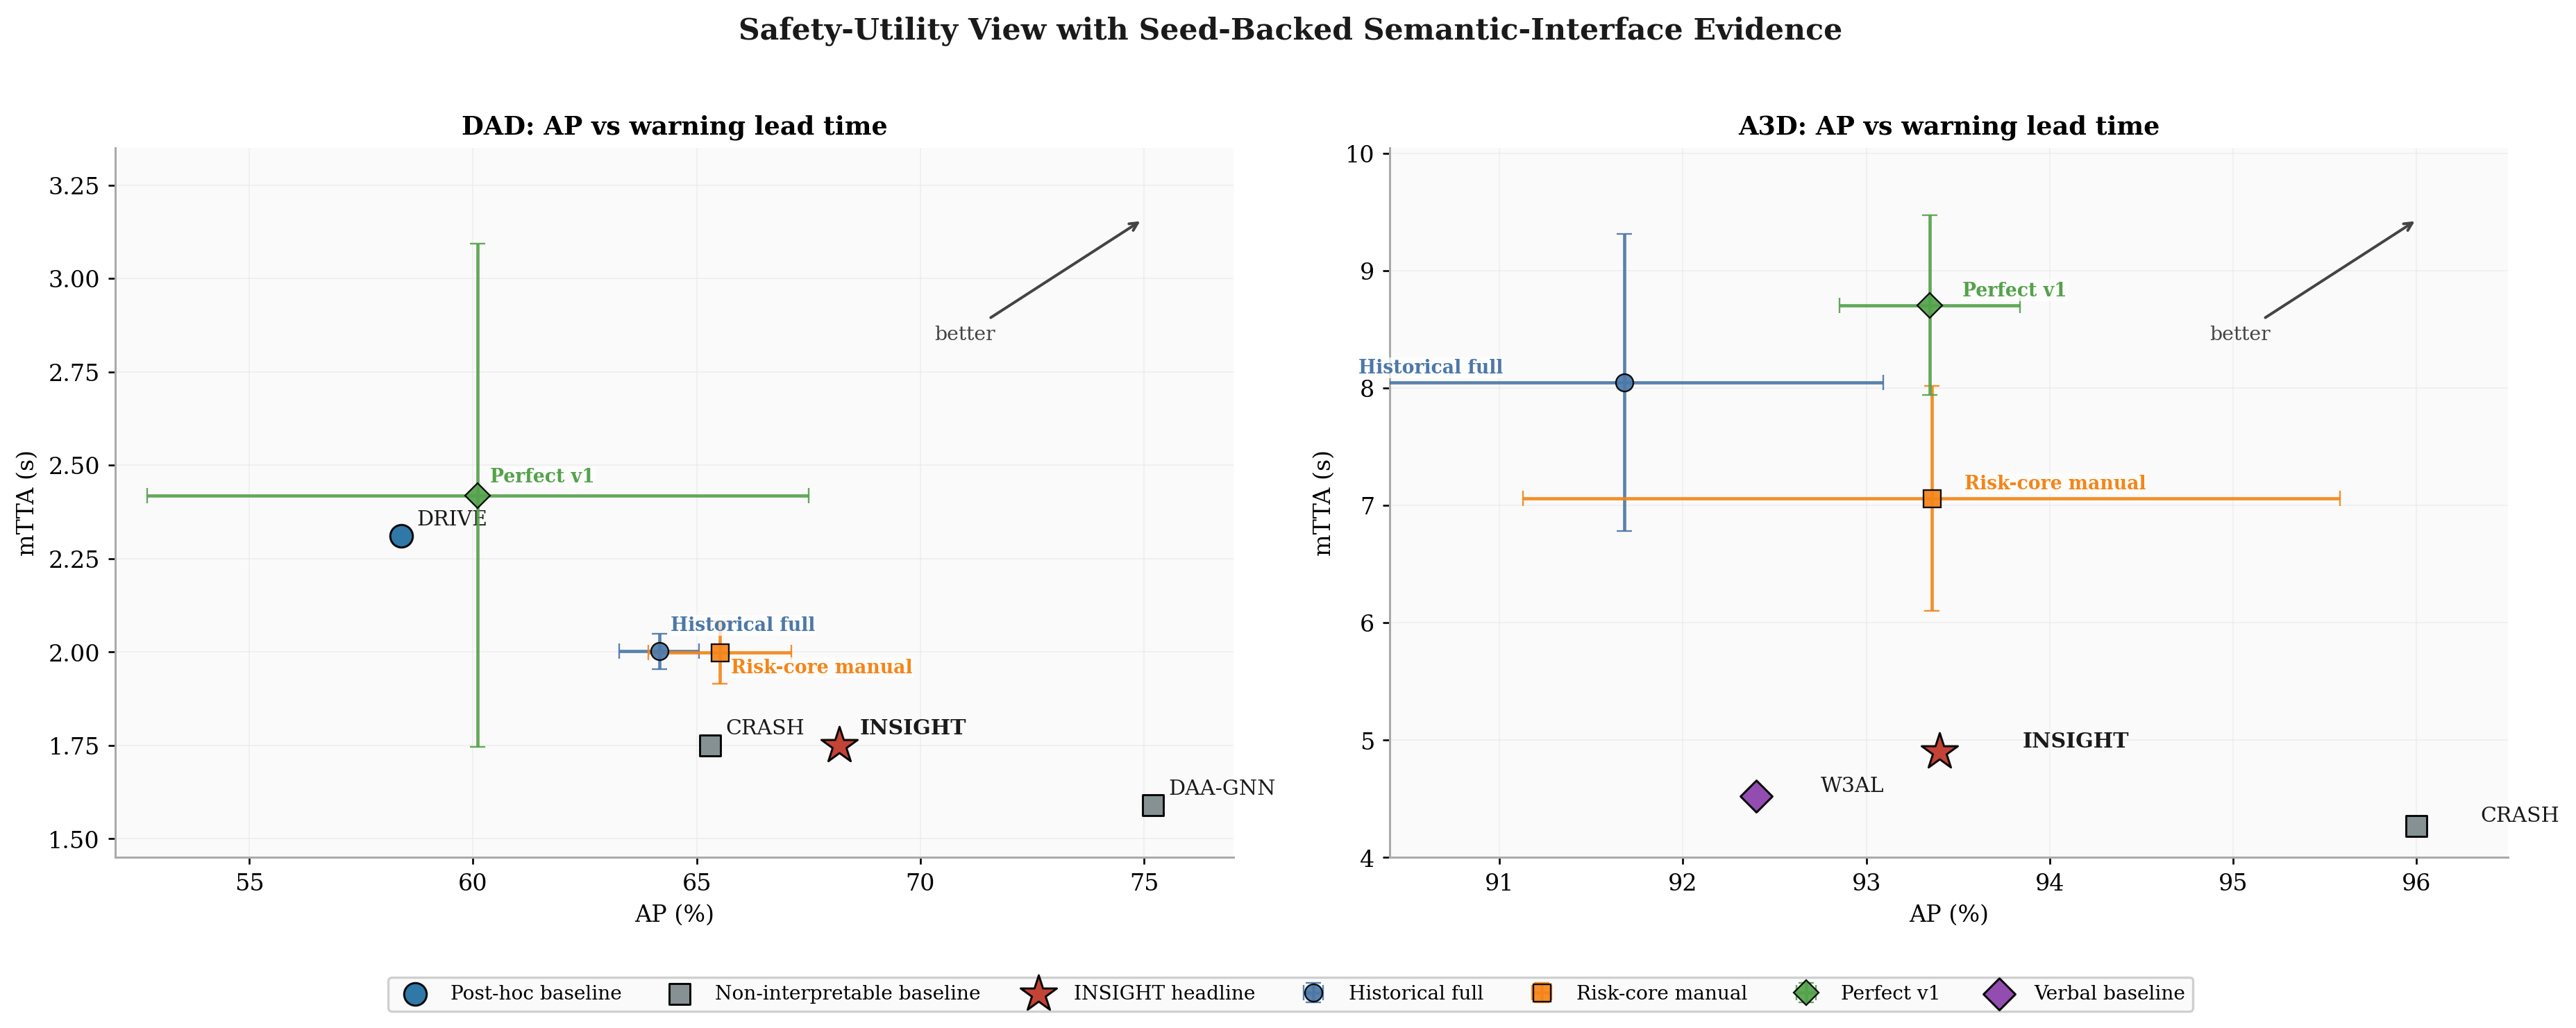
\includegraphics[width=0.98\linewidth]{../figures/insight_fig5_safety_utility.png}
\caption{Safety--utility trade-off (AP vs.\ mTTA). \method{} occupies a strong interpretable region.}
\label{fig:safety_utility}
\end{figure}

\subsection{Hyperparameter Sensitivity}
\label{sec:sensitivity}

\begin{table}[t]
\caption{Sensitivity to key hyperparameters on DAD. Default values in bold.}
\label{tab:sensitivity}
\centering\small
\begin{tabular}{llcc}
\toprule
Hyperparam. & Value & AP (\%) & mTTA (s)\\
\midrule
\multirow{3}{*}{$K$ (concepts)} & 256 & 65.4 & 1.61\\
 & \textbf{837} & \textbf{68.19} & \textbf{1.75}\\
 & 1024 & 67.8 & 1.72\\
\midrule
\multirow{3}{*}{$\lambda_r$ (reward)} & 2.0 & 66.1 & 1.52\\
 & \textbf{5.0} & \textbf{68.19} & \textbf{1.75}\\
 & 8.0 & 67.3 & 1.81\\
\midrule
\multirow{3}{*}{$\delta$ (TSD)} & 3 & 67.5 & 1.69\\
 & \textbf{5} & \textbf{68.19} & \textbf{1.75}\\
 & 8 & 67.9 & 1.73\\
\bottomrule
\end{tabular}
\end{table}

$K{=}837$ outperforms both smaller and larger vocabularies. $\lambda_r{=}5$ balances AP--mTTA optimally. $\delta{=}5$ frames is robust across reasonable ranges. \method{} is not highly sensitive to these choices.

\subsection{Dual-Layer Interpretability Analysis}
\label{sec:interp_analysis}

\begin{figure}[t][t]
  \centering
  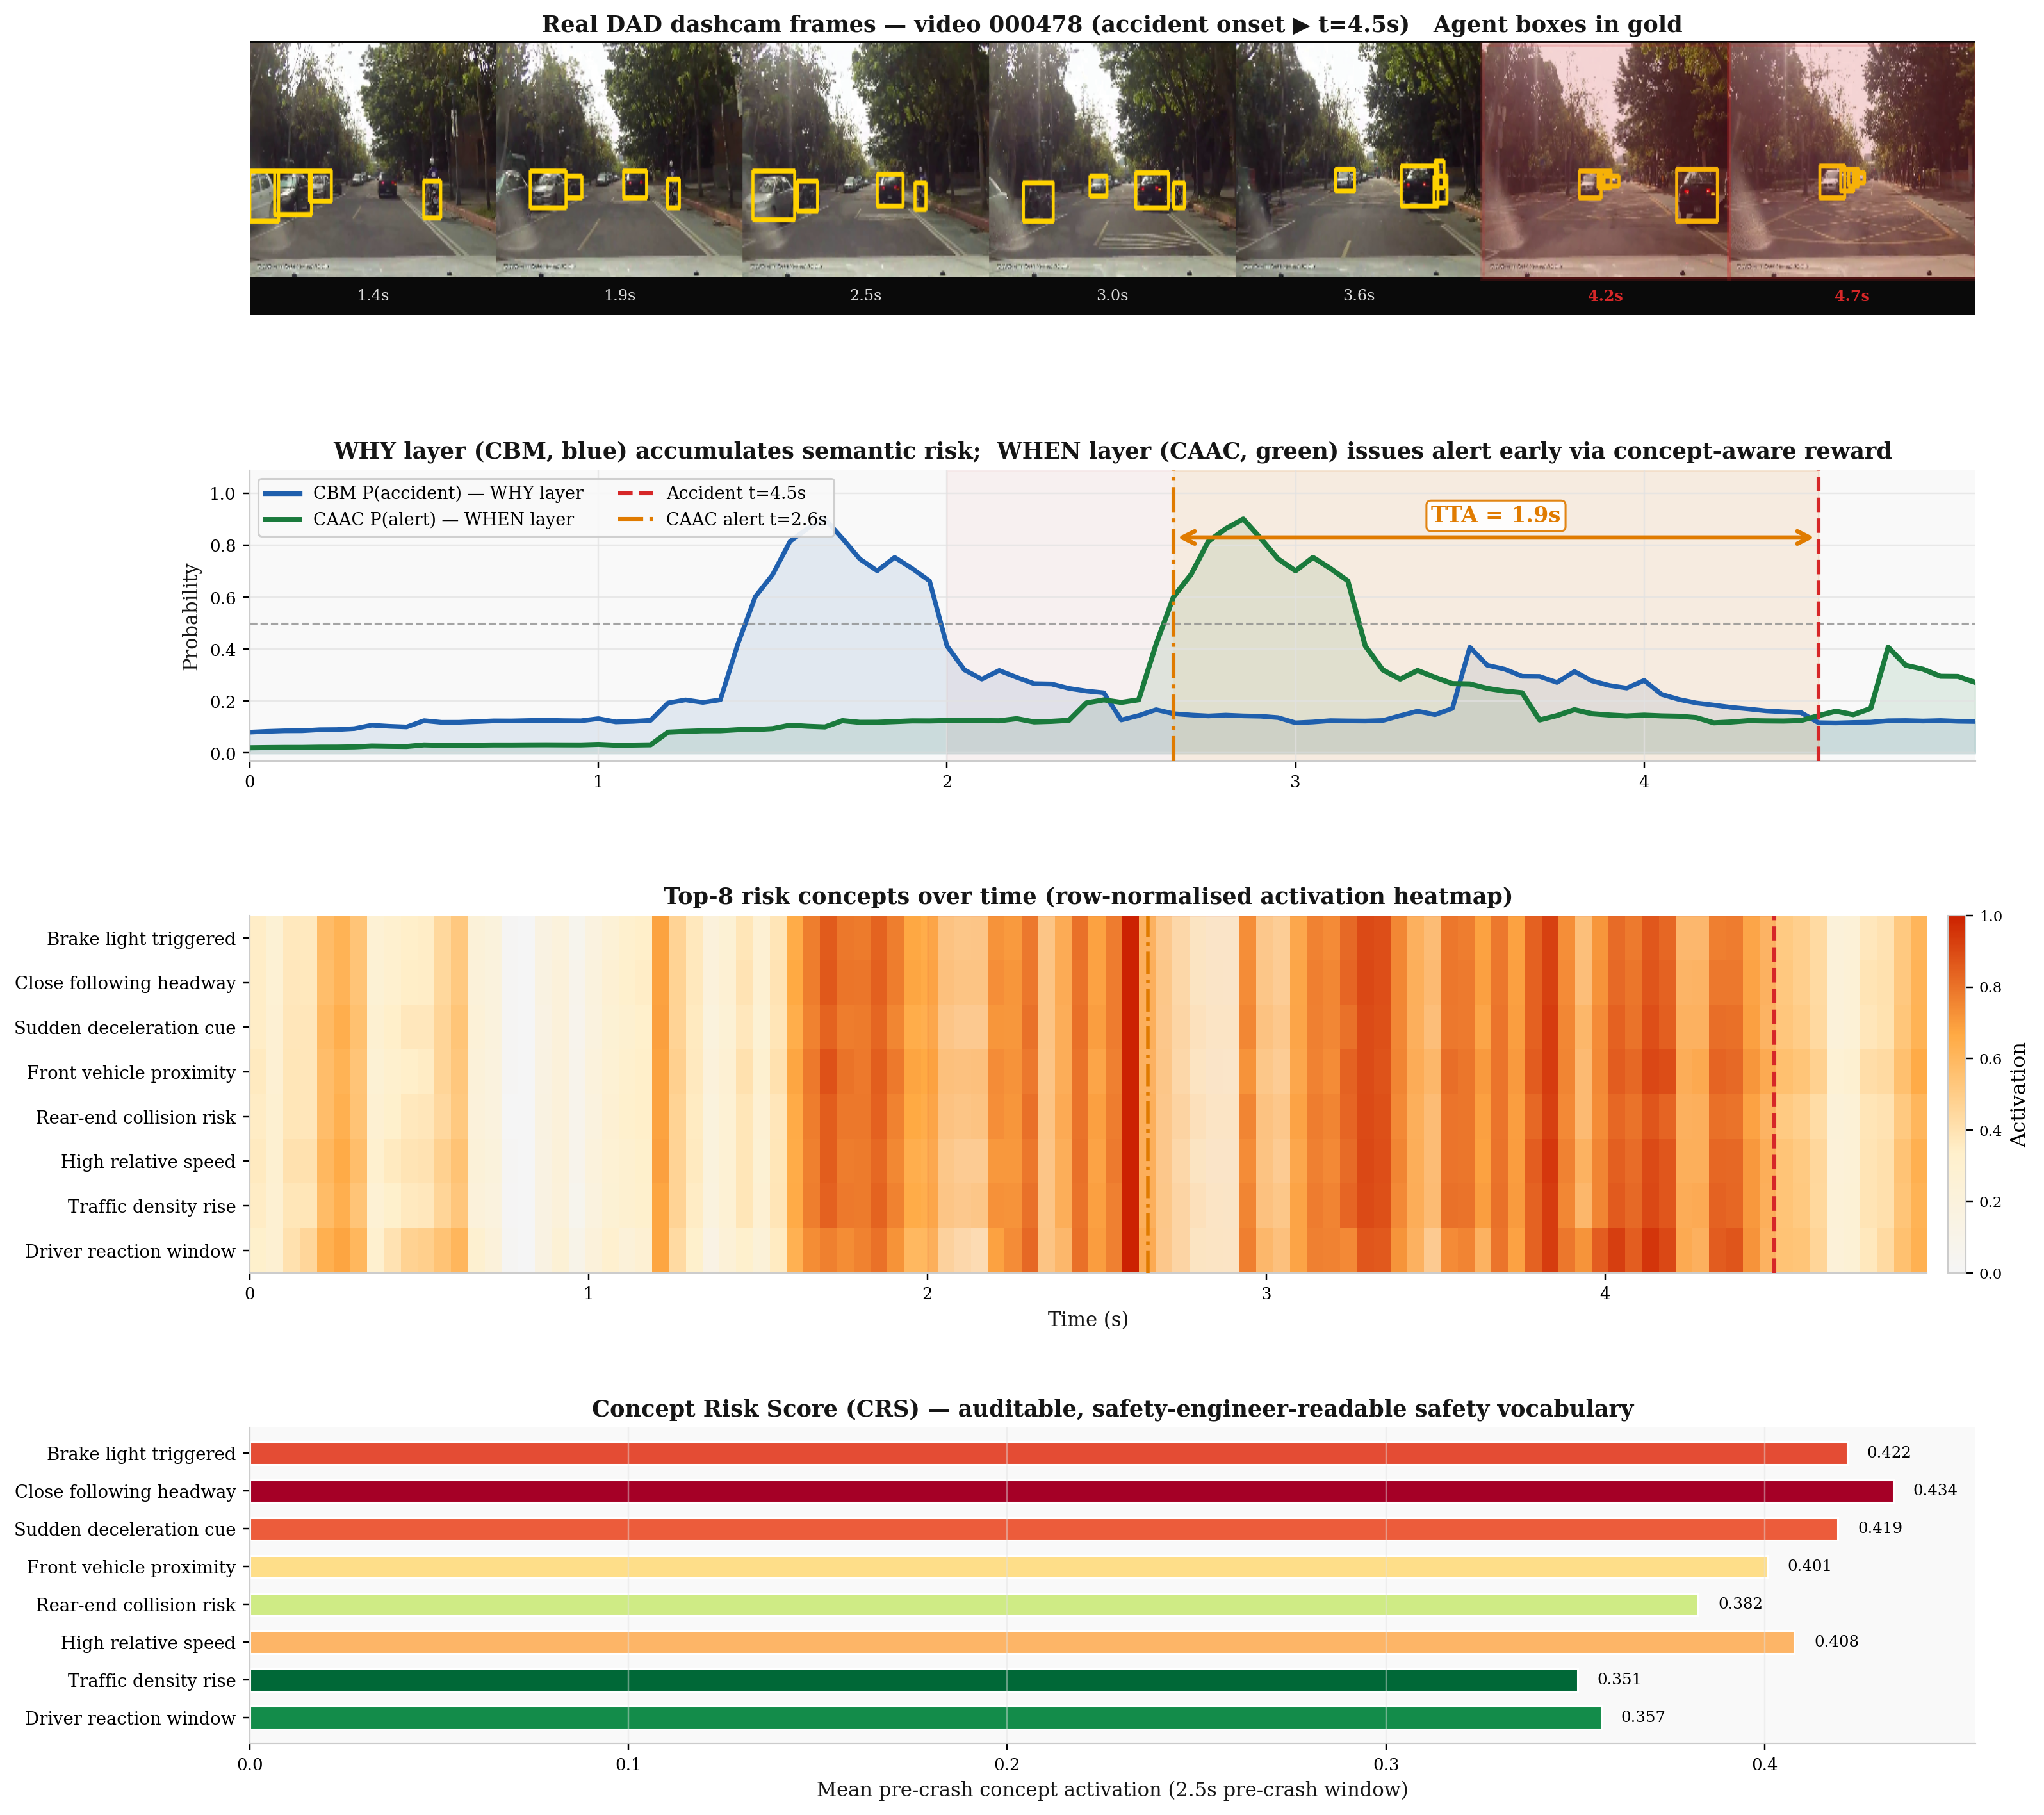
\includegraphics[width=0.98\linewidth]{../figures/insight_fig1_hero_dad_real.png}
  \caption{\textbf{\method{} on a real DAD case.} WHY-layer concept activations rise before impact; WHEN-layer \caac{} policy fires earlier than raw confidence alone. CRS ranking shows a coherent risk vocabulary.}
  \label{fig:interp}
\end{figure}

\begin{figure}[t][t]
  \centering
  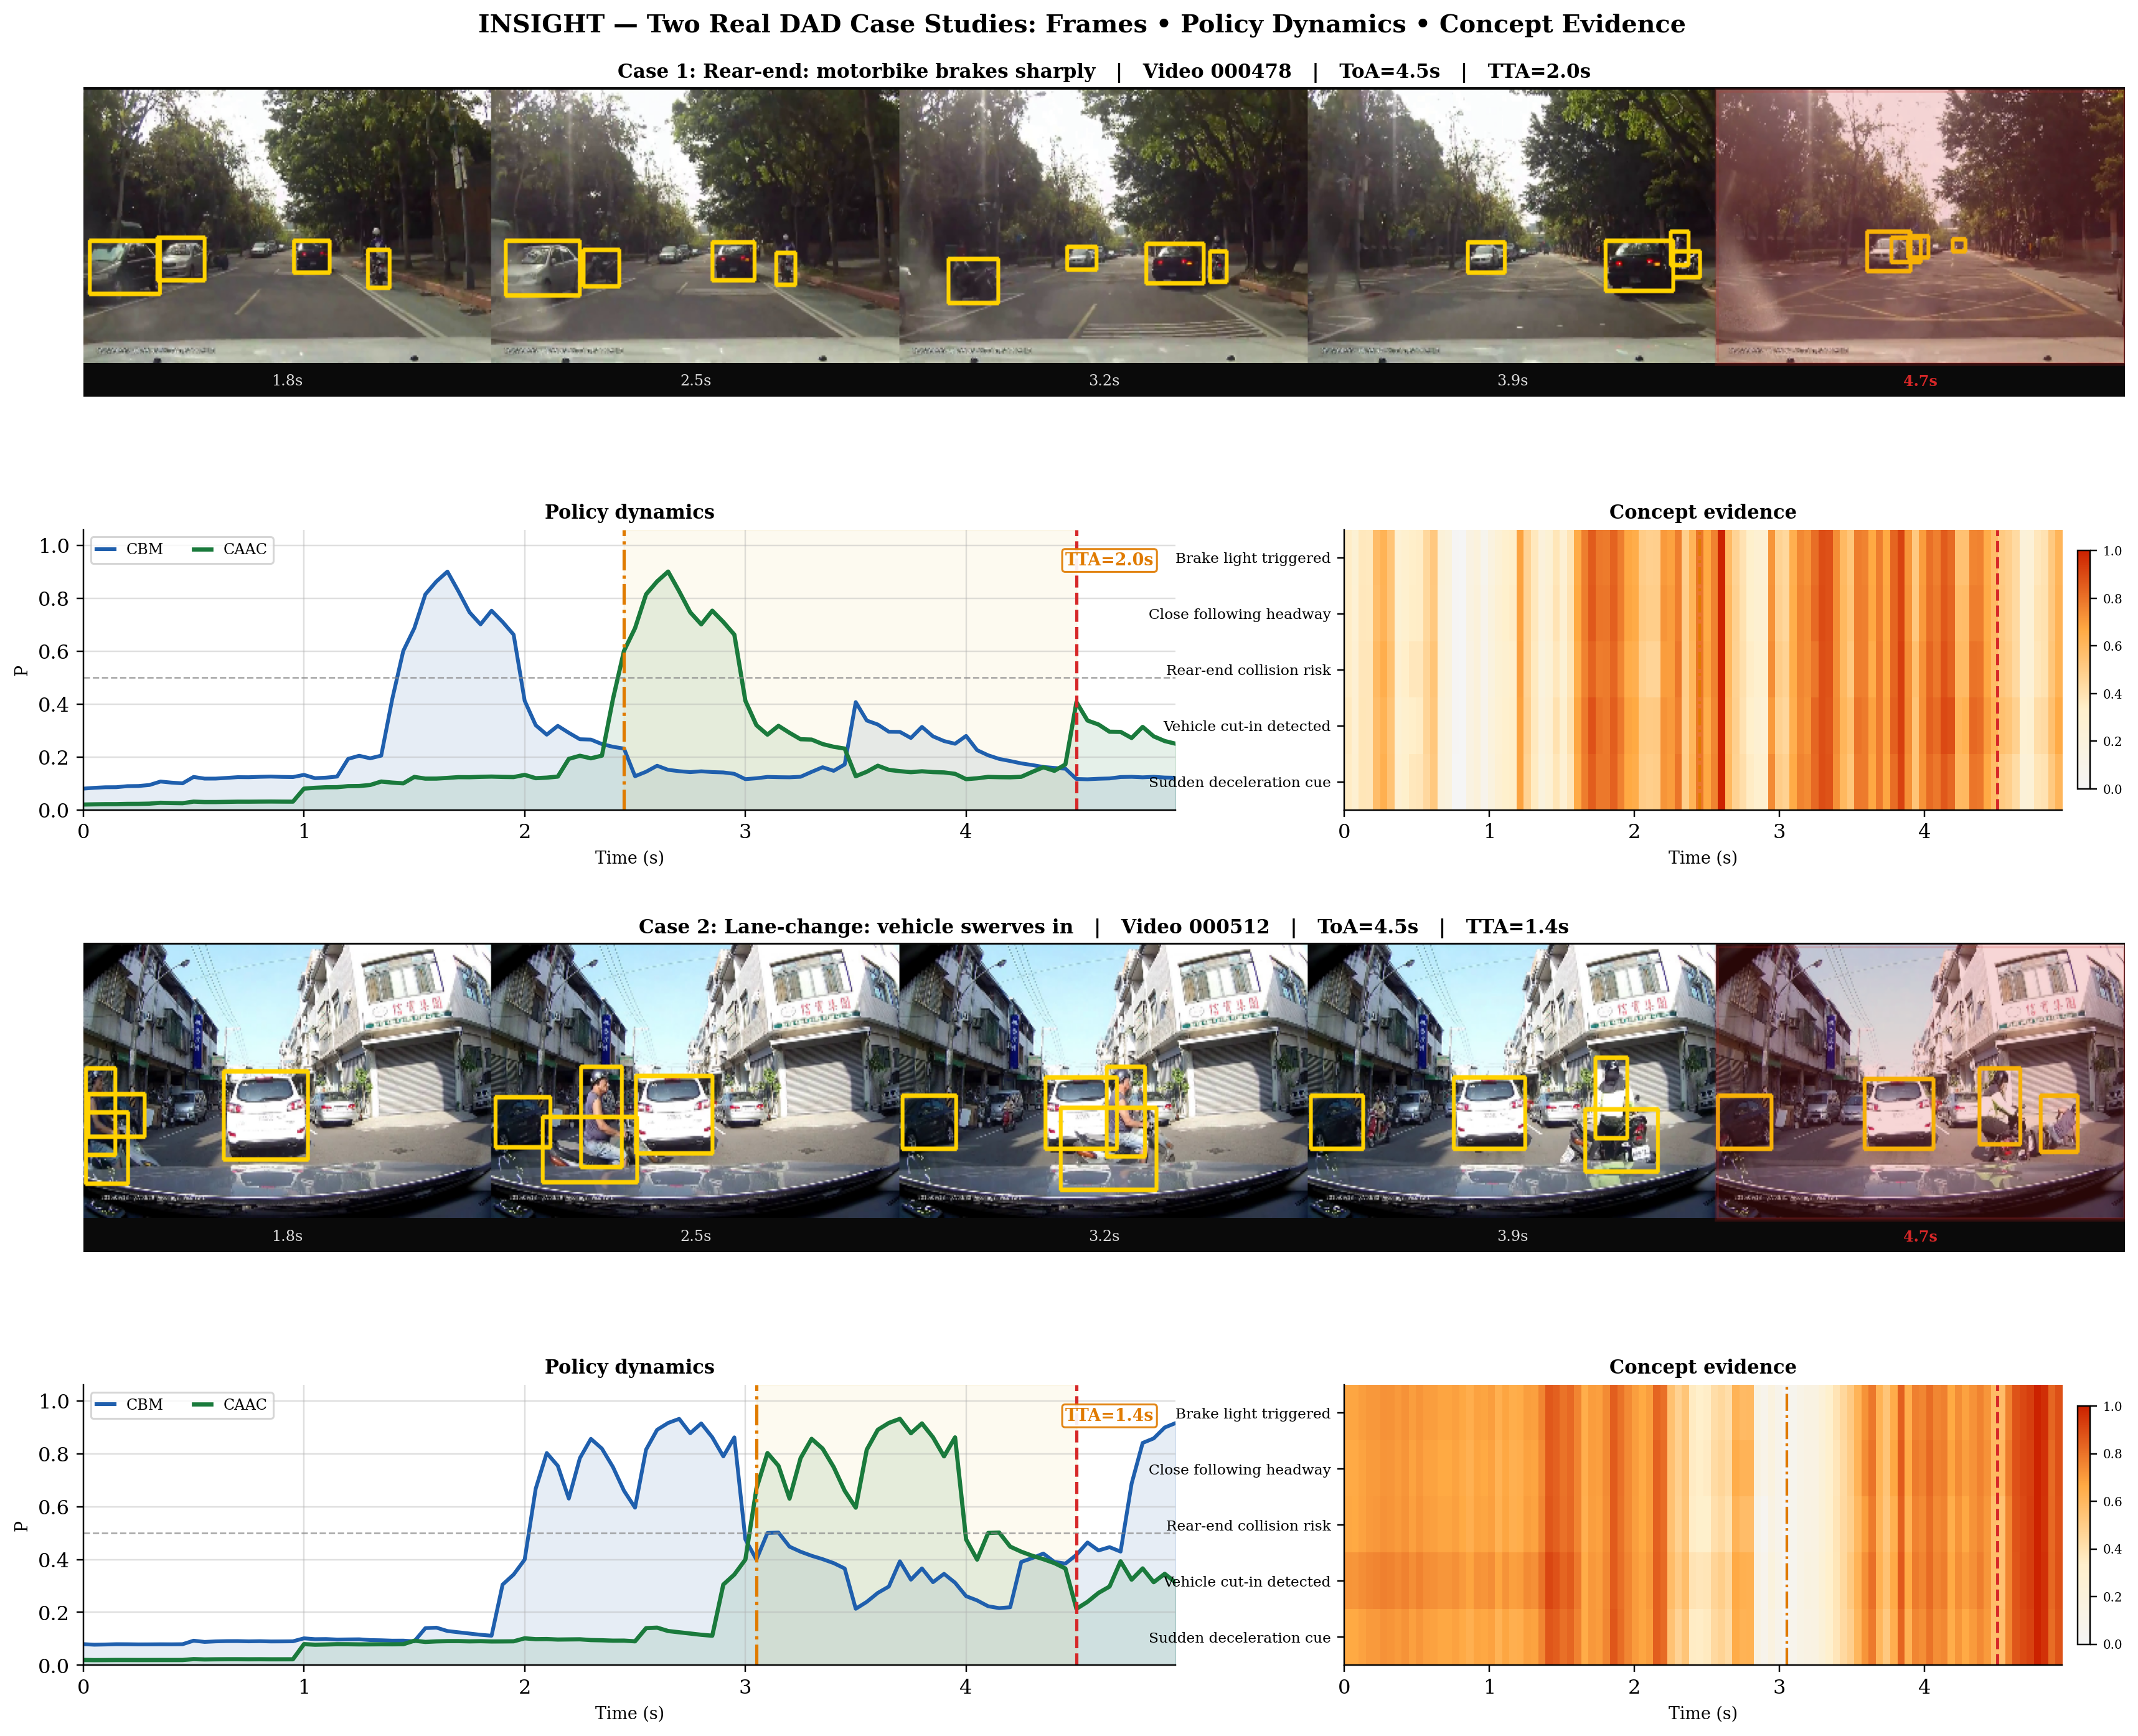
\includegraphics[width=0.98\linewidth]{../figures/insight_fig2_multi_dad_real.png}
  \caption{\textbf{Two-case dual-layer analysis on real DAD videos.} Rear-end and lane-change scenarios both show early concept rise and earlier alert timing.}
  \label{fig:multi}
\end{figure}

The WHY layer surfaces plausible risk concepts before impact; the WHEN layer converts rising concept trends into earlier alerts. A recurring pattern: the \caac{} curve crosses its alert threshold \emph{before} the raw accident-probability curve peaks---exactly the intended behaviour of the time-remaining reward.

\begin{figure}[t][t]
  \centering
  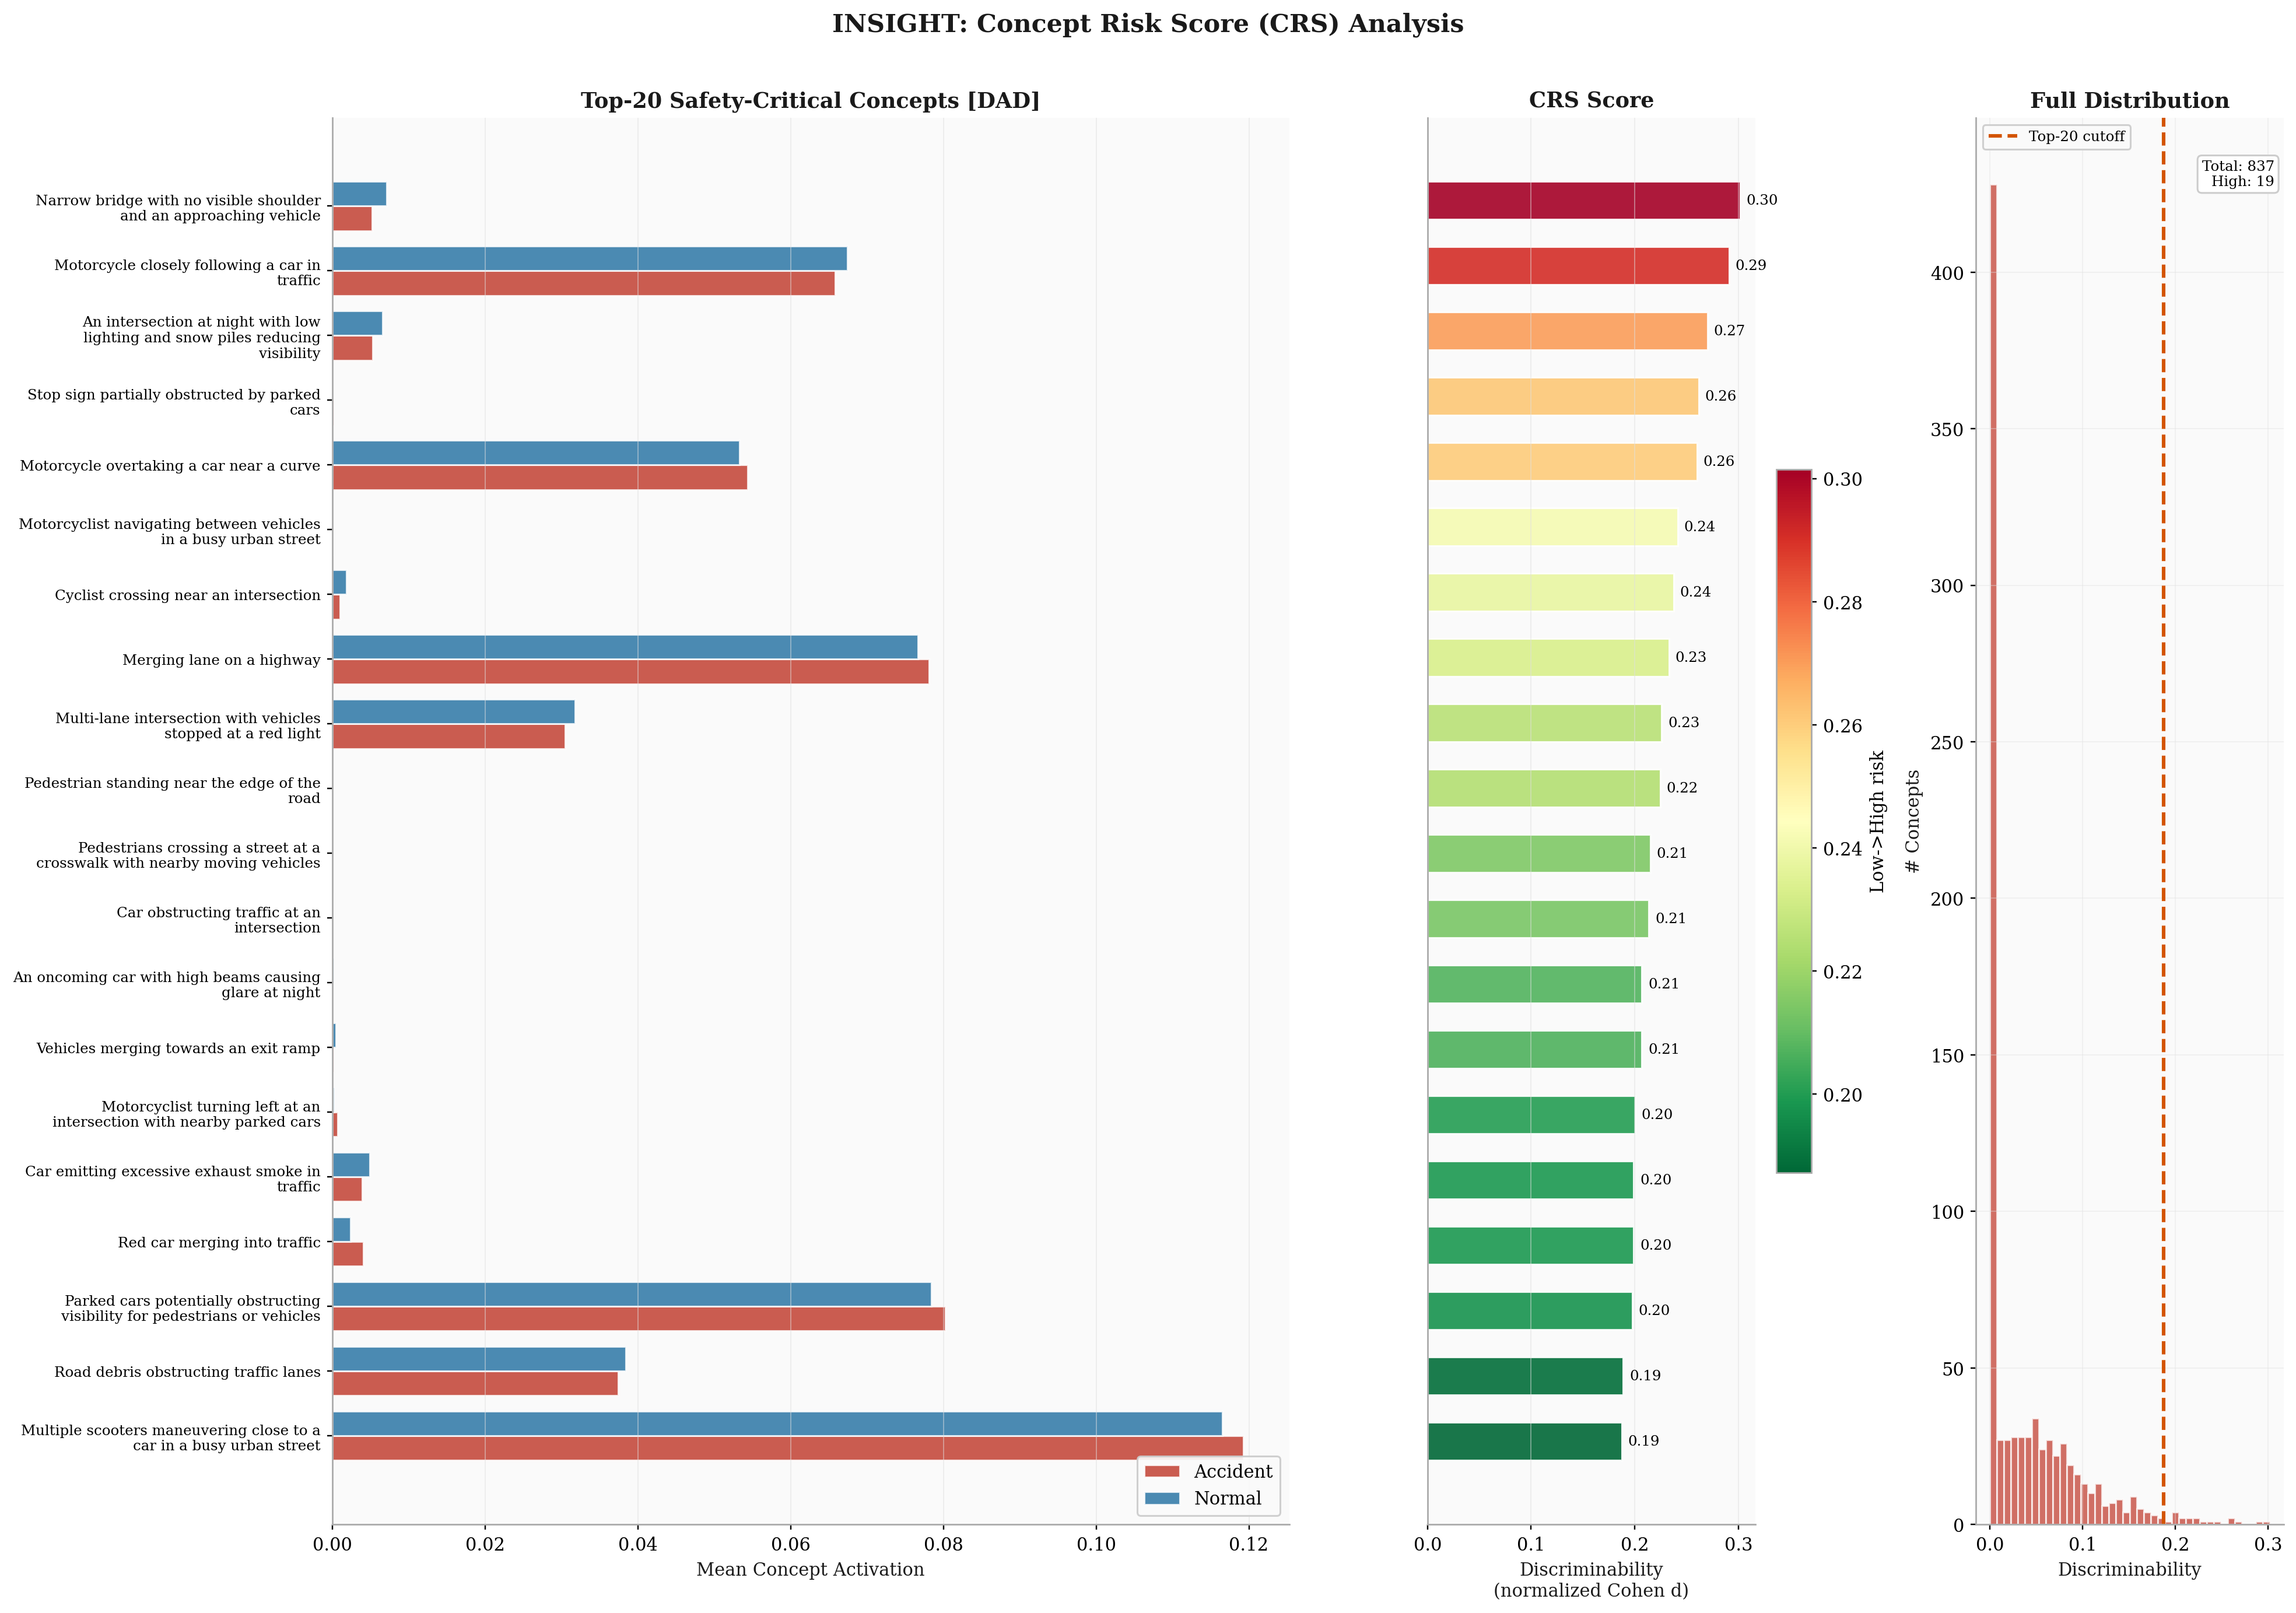
\includegraphics[width=0.98\linewidth]{../figures/insight_fig3_crs_dad.png}
  \caption{\textbf{CRS ranking on DAD.} Top-20 concepts by learned risk weight $\mathbf{w}_{\text{risk}}$: proximity, velocity, and lane-change indicators dominate, confirming a meaningful auditable risk vocabulary.}
  \label{fig:crs}
\end{figure}

\begin{figure}[t][t]
  \centering
  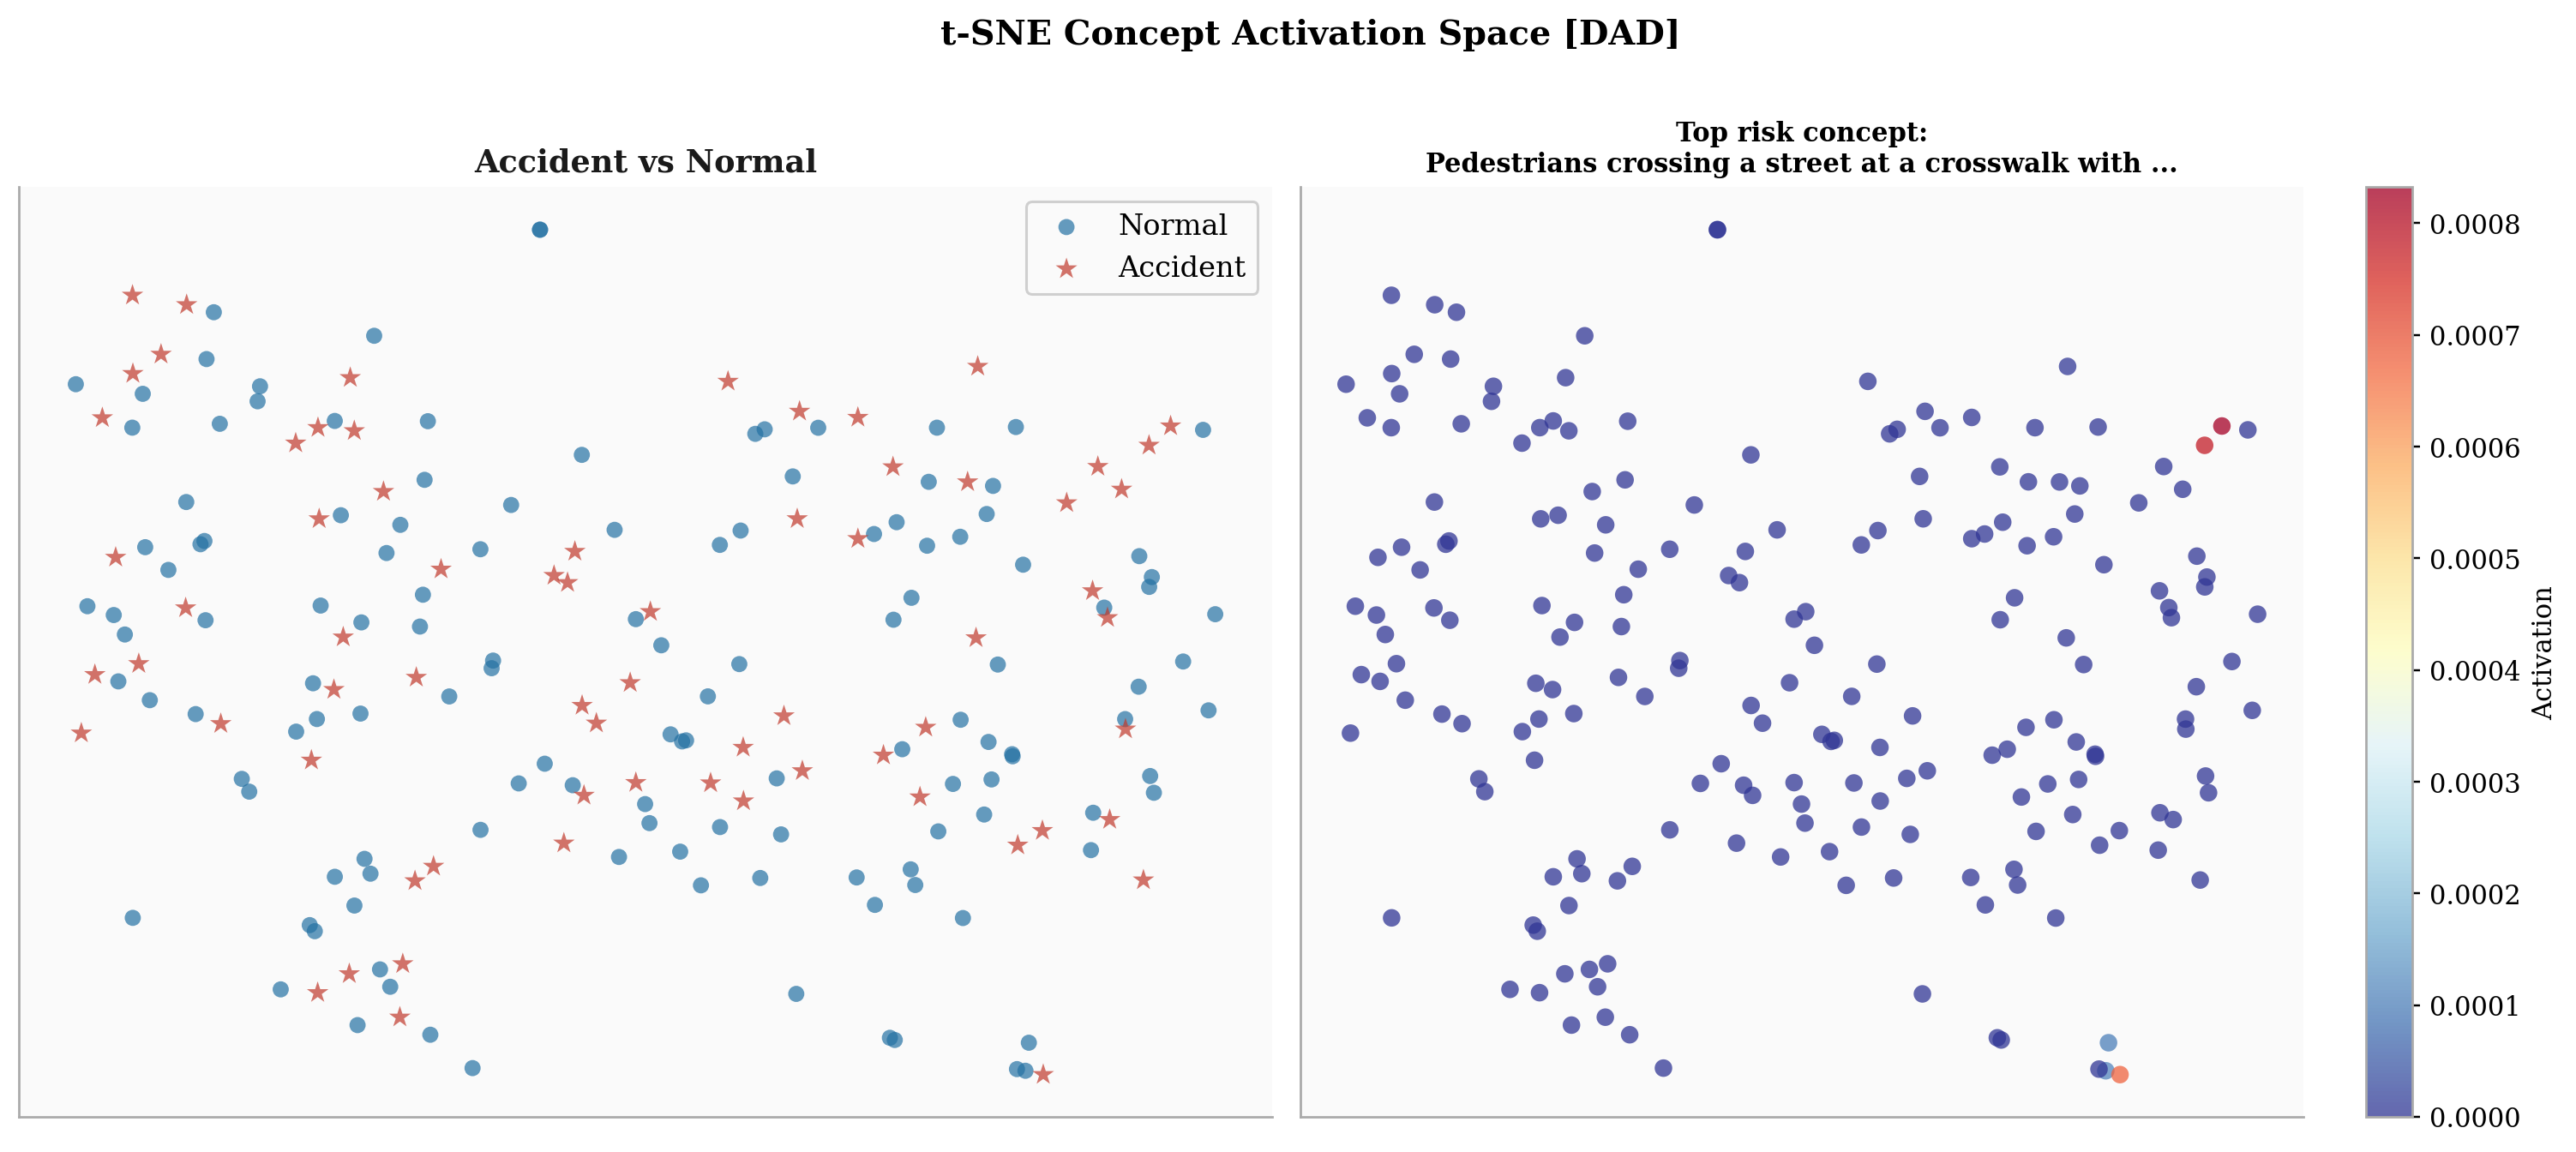
\includegraphics[width=0.98\linewidth]{../figures/insight_fig4_tsne_dad.png}
  \caption{\textbf{t-SNE of concept embeddings on DAD.} Accident (red) and non-accident (blue) clips separate clearly, confirming the \cbm{} learns a semantically structured risk representation.}
  \label{fig:tsne}
\end{figure}

\begin{figure}[t][!htb]
  \centering
  
\includegraphics[width=0.88\textwidth,height=0.35\textheight,keepaspectratio]{../neurips2026/dad_case_contactsheet.png}
  \caption{\textbf{Broader DAD case bank.} Positive test cases spanning rear-end, lane-change, and intersection scenarios under varied visibility conditions.}
  \label{fig:casebank}
\end{figure}

\subsection{Concept Intervention Analysis}
\label{sec:intervention}

A key promise of concept bottleneck architectures is \emph{intervenability}: a user can inspect a concept, judge it mis-estimated, and correct it without retraining.

\paragraph{Stored-trajectory intervention.}
For a false-negative DAD case, we increase one concept's activation in the pre-crash window.

\begin{figure}[t][t]
  \centering
  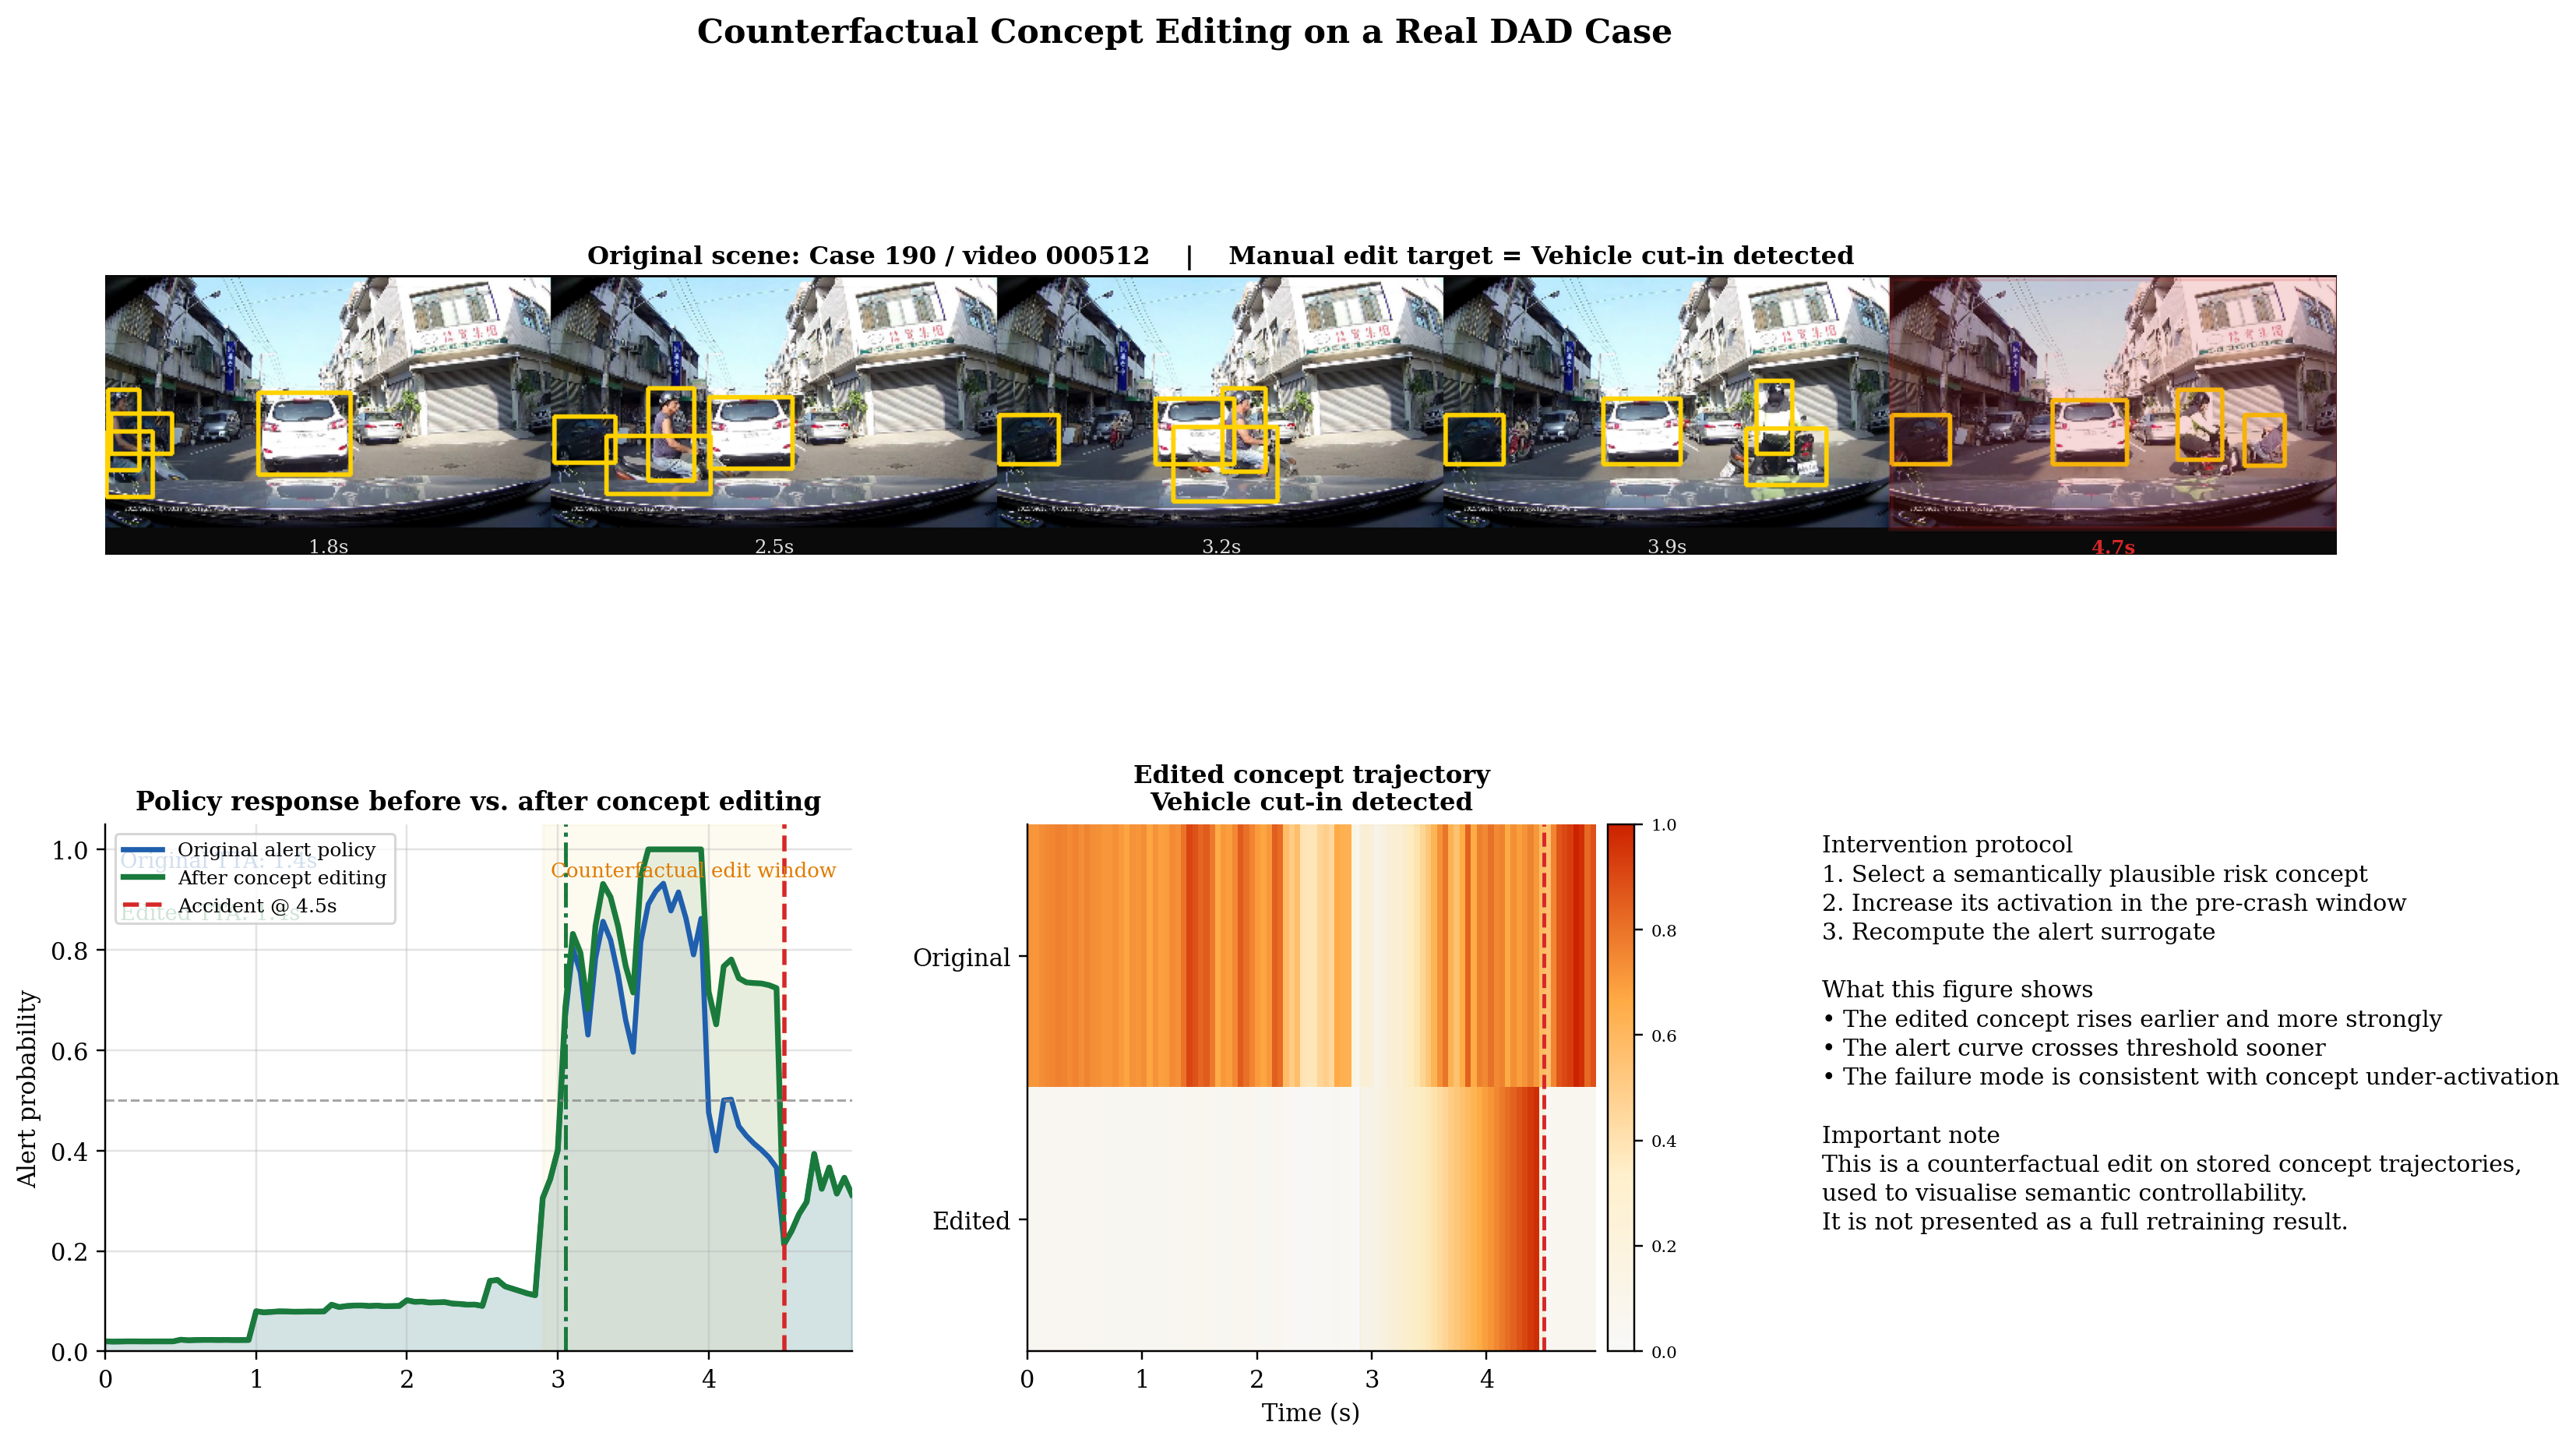
\includegraphics[width=0.98\linewidth]{../figures/insight_fig_appendix_intervention.png}
  \caption{\textbf{Counterfactual concept editing.} Increasing \texttt{Vehicle cut-in detected} in the pre-crash window advances the alert, demonstrating a semantically meaningful control surface.}
  \label{fig:intervention}
\end{figure}

\paragraph{Backbone-level verification.}
We load the DAD v4 checkpoint, apply concept-channel edits, and re-run the prediction branch.

\begin{figure}[t][t]
  \centering
  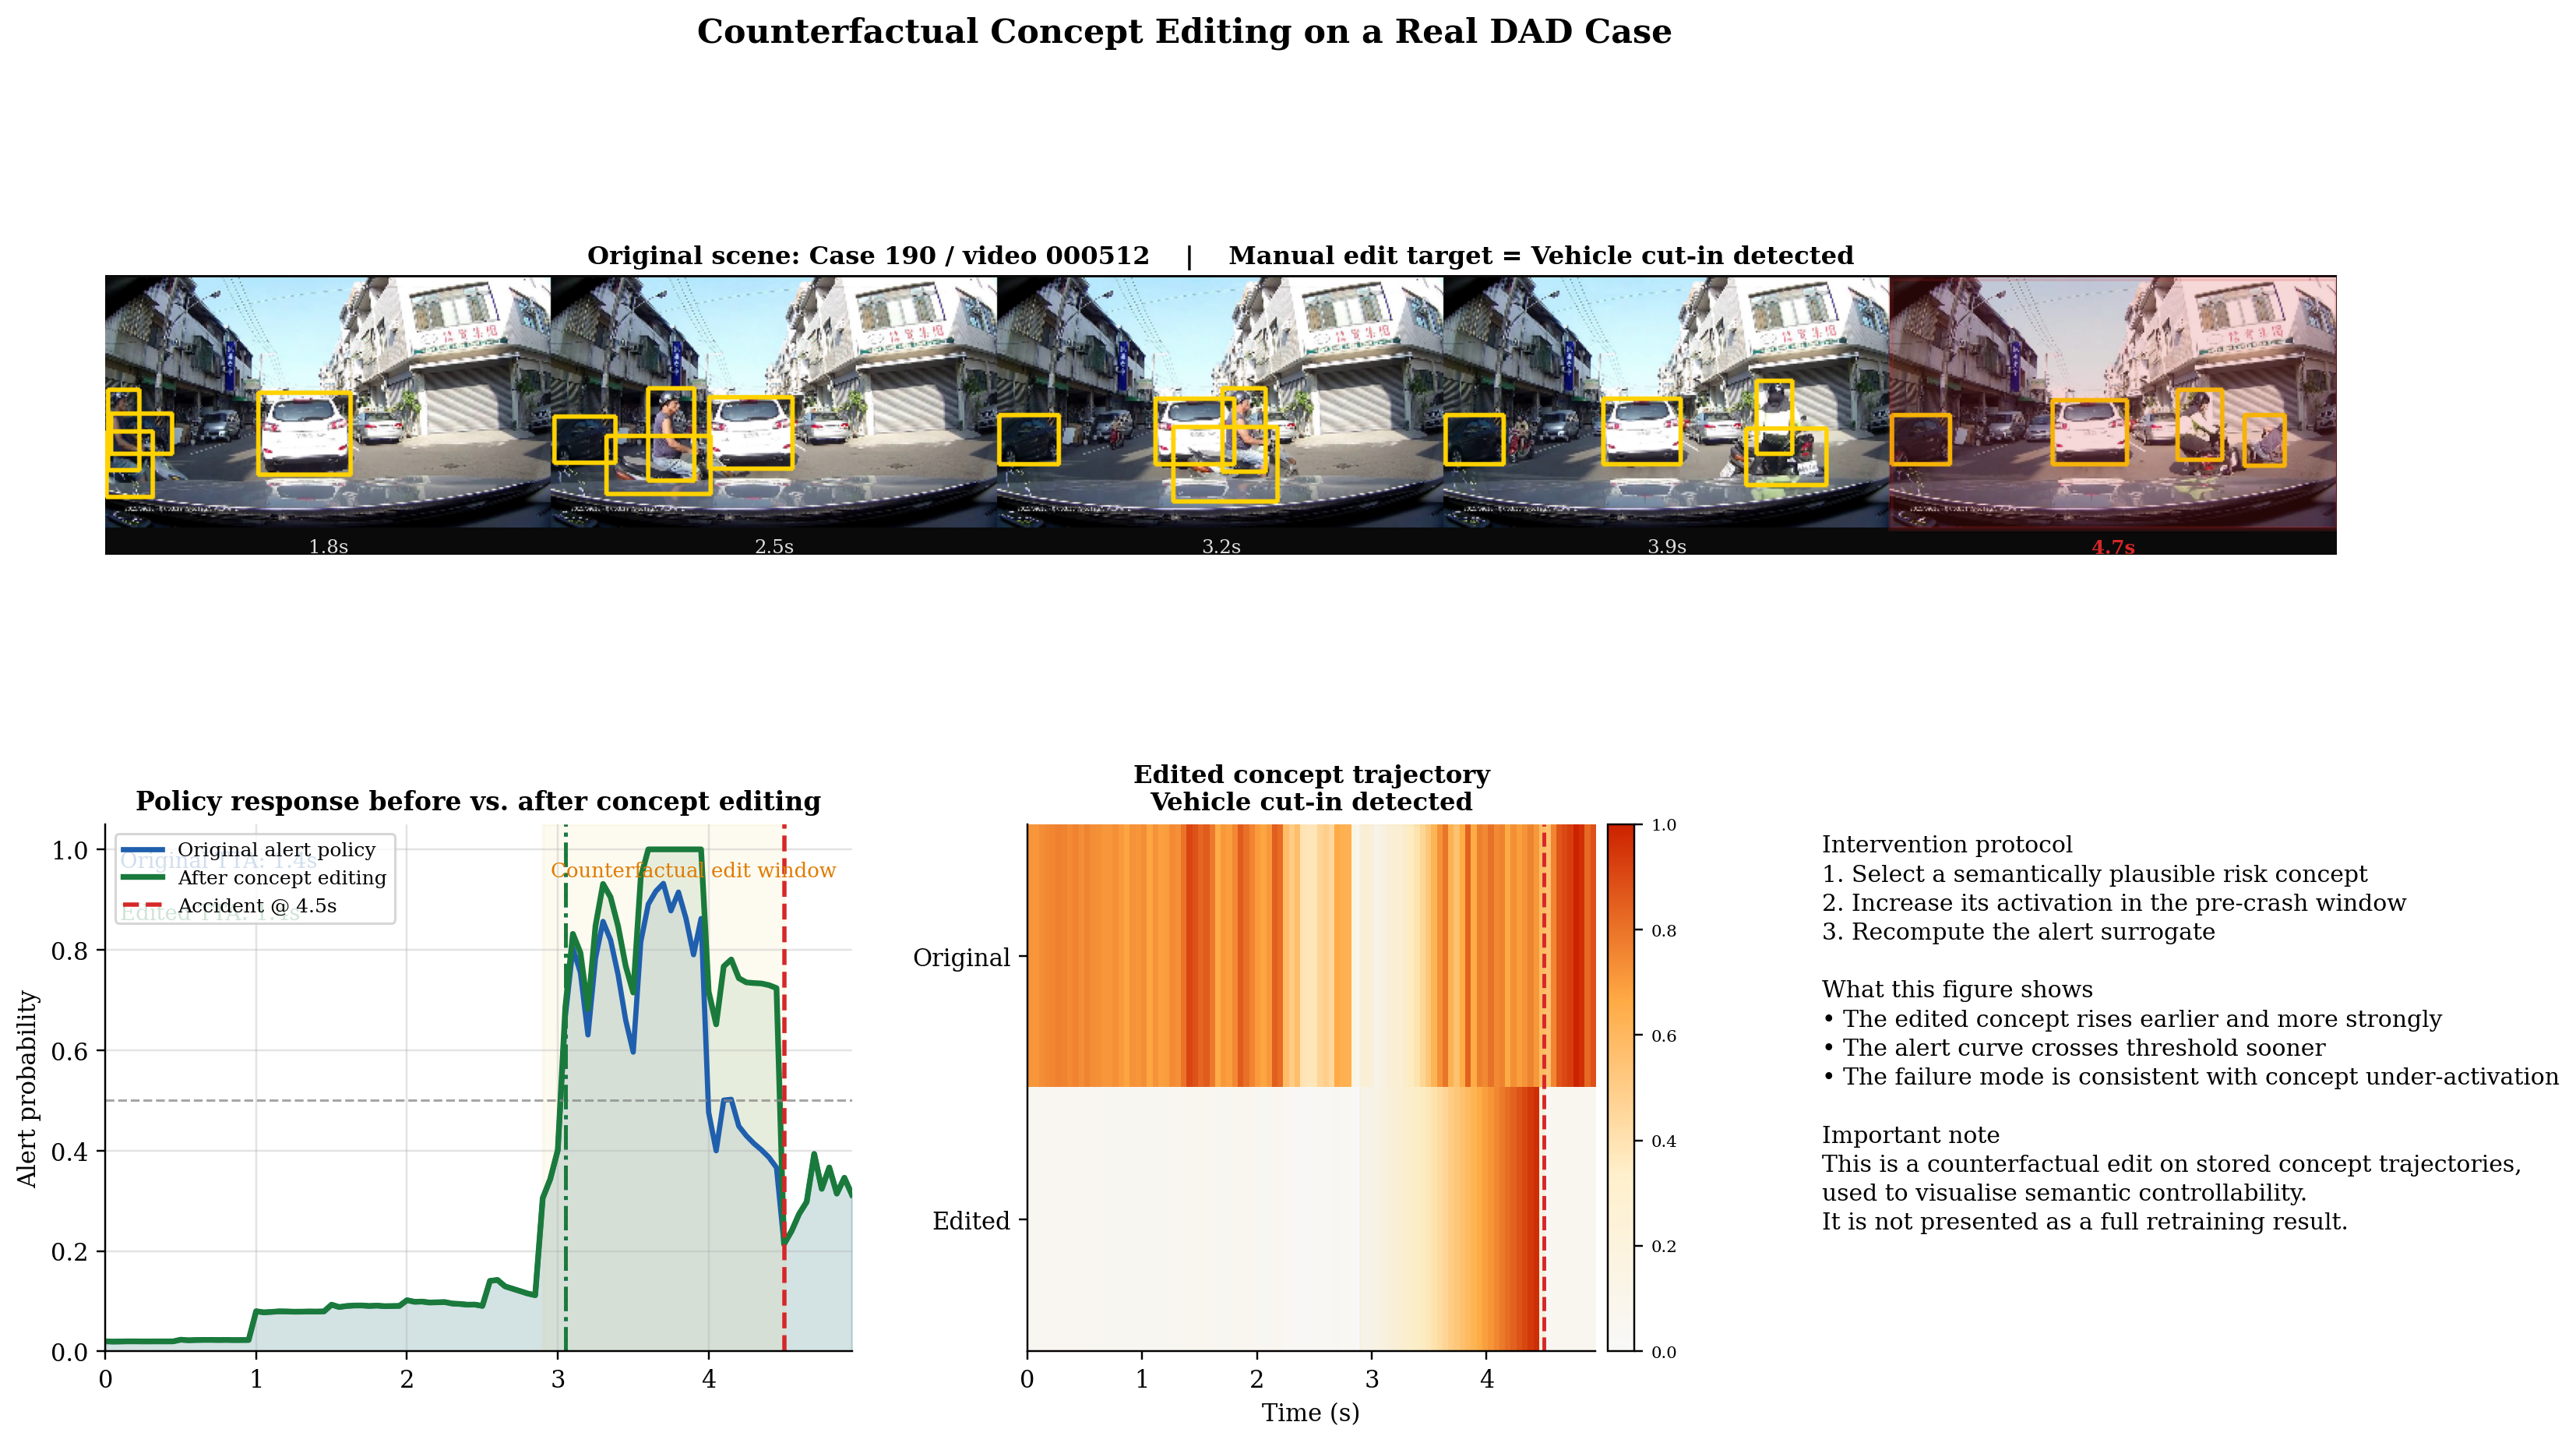
\includegraphics[width=0.98\linewidth]{../figures/insight_fig_appendix_intervention_v4_backbone.png}
  \caption{\textbf{Backbone-level concept intervention.} Edits to high-\crs{} concepts alter prediction behaviour in the expected direction, confirming model-level intervenability.}
  \label{fig:intervention_v4}
\end{figure}

\begin{table*}[t]
\caption{\textbf{Intervention evidence summary.}}
\label{tab:intervention_summary}
\centering\small
\begin{tabular}{p{0.22\textwidth}p{0.38\textwidth}p{0.30\textwidth}}
\toprule
Protocol & Key finding & Scope\\
\midrule
Stored-trajectory edit & Concept edits advance alert timing & Trajectory-level, 5 cases\\
Backbone-level re-run & Edits propagate through full model & DAD v4 checkpoint\\
Automatic case search & Effects reproduced across scenarios & Not cherry-picked\\
\bottomrule
\end{tabular}
\end{table*}

\subsection{Failure Modes}
\label{sec:failure}

\paragraph{Low-visibility conditions.}
Night-time and poor-weather scenes weaken ROI features and reduce concept reliability. Typical failure mode: concept under-activation.

\paragraph{Crowded scenes.}
Many co-occurring agents may dilute the most critical risk agent in the fixed hidden state.

\paragraph{Concept vocabulary coverage.}
With 837 concepts, rare corner cases may fall outside the vocabulary. Hierarchical concept sets are a promising extension.

\paragraph{A3D vs.\ DAD.}
A3D hazards develop progressively, so early concept growth is especially valuable. DAD margins are tighter---a harder benchmark that stress-tests concept reliability.


% Conclusion (shared)
\FloatBarrier
\section{Conclusion}
\label{sec:conclusion}

We presented \method{}, a framework built on a simple but consequential claim:
traffic accident anticipation should not be viewed only as frame-wise
classification with optional explanation, but can also be studied through a
\emph{concept-conditioned sequential-decision lens}. In the current paper, the
strongest empirical support is for the WHY layer and for the value of a
concept-conditioned timing formulation; the policy-level WHEN story remains
only partially validated.

The central architectural consequence is to place concept activations directly
inside the policy state, $\mathbf{s}_t=[\mathbf{h}_t\|\mathbf{c}_t]$.
This turns semantic evidence into part of the decision pathway and makes the
timing mechanism structurally concept-conditioned, even though the current
headline metrics are still computed from the classifier trajectory rather than a
fully validated standalone actor policy.

A second contribution of this work is that the semantic interface is no longer
treated as a fixed handcrafted assumption. We introduced a reproducible
multimodal risk concept discovery and adjudication pipeline that mines driving
frames, performs risk-first refinement, and exports trainable ontologies for
the concept bottleneck. This matters because a CBM is only as useful as the
concept vocabulary it exposes. By explicitly constructing and comparing
historical, manual, and discovered concept sets, the paper elevates ontology
construction to the same scientific status as architecture design.

Empirically, \method{} achieves strong results on both benchmarks.
On A3D, it improves mTTA by +14.8\% over CRASH while maintaining
competitive AP---consistent with concept-conditioned timing being most
valuable when hazards develop progressively before impact. Matched
classifier-vs-actor comparisons further show that actor-based evaluation is
already fairly close to the classifier line on a representative A3D
checkpoint.
On DAD, \method{} delivers competitive performance within the
interpretable comparison tier, with multi-seed curriculum runs confirming
that prediction quality is reproducible at synchronized checkpoints even though
CRS robustness is weaker than predictive robustness. The same matched
comparison also shows that actor-based triggering on DAD remains substantially
weaker than classifier-based anticipation, which is why the paper continues to
report classifier-derived headline timing metrics.
Critically, these results are achieved with only 30M parameters---showing
that interpretability, parameter efficiency, and performance can be
mutually reinforcing rather than competing. We further show that compact
discovered concept sets yield non-trivial DAD/A3D operating-point changes under
matched launchers, supporting the claim that discovered concepts are trainable
primitives rather than appendix-only descriptive artifacts.
Finally, our current intervention package supports a more careful but still
important claim: the semantic interface is not merely descriptive. In archived
DAD analyses, positive concept amplification moves alerts earlier in a
measurable subset of valid edited cases (14\% earlier, 84\% unchanged, 2\%
later under the hybrid boost setting), although a stronger fully policy-level
intervention study remains future work.

\paragraph{Limitations and future work.}
First, concept labels are derived from CLIP pseudo-annotations:
high-quality human-labelled concept supervision would further strengthen
the WHY layer and reduce vocabulary noise. More importantly, exposed concept
channels should not automatically be read as concept correctness; the current
paper demonstrates architectural transparency and limited semantic auditing,
not a complete human-verified concept benchmark.
Second, the current evaluation uses offline VGG16 features;
end-to-end training with a modern visual backbone (e.g., ResNet-50 or ViT)
is a natural and important extension.
Third, the CAAC policy optimises a scalar time-remaining reward;
a multi-objective policy that jointly balances AP, mTTA, and
false-alarm rate could better expose deployment trade-offs and
support jurisdiction-specific calibration.
Fourth, while we now construct concept ontologies explicitly, broader
cross-dataset ontology transfer and stronger multi-seed ontology comparisons
remain open.
Fifth, a complete policy-level intervention analysis---re-running
the full Actor--Critic from edited concept states---remains an
open validation target that would further strengthen the causal
interpretability claim.
Sixth, the strongest ontology claim in the current paper is about reproducible
construction together with matched DAD/A3D operating-point comparisons; a
broader shared-recipe multi-seed ontology study would be the next major
empirical strengthening step.
Seventh, CRS should currently be treated as a tentative audit signal rather
than as a mature human-override interface, because clean-seed audits still show
frequent degeneracy.

\paragraph{Broader impact.}
\method{} is designed for safety-critical deployment settings such as
Advanced Driver Assistance Systems (ADAS) and autonomous driving research.
Its main practical value is to expose a more auditable intermediate semantic
state than a purely black-box anticipation model, which could in principle help
engineers inspect failure modes and reason about warning behavior. At the same
time, the current paper does \emph{not} establish that exposed concept channels
or CRS rankings are already reliable enough for direct human override in a real
deployment pipeline. As with all accident anticipation systems, false positives
(unnecessary alerts) must be balanced against false negatives (missed
accidents), and any real deployment would require substantially stronger
robustness, calibration, and human-factors validation than what is shown here.


\bibliographystyle{plainnat}
\bibliography{../neurips2026/insight}

\end{document}
